%% ****** Start of file rsitemplate.tex ****** %
%%
%%   This file has been edited from the original source file.
%%	 The original file is part of the revtex4-1 package indicated below.
%%   Version 4.1 of 9 October 2009.
%%
%
% This is a template for producing documents for use with 
% the REVTEX 4.1 document class and the RSI substyle.
% 
% Copy this file to another name and then work on that file.
% That way, you always have this original template file to use.


\documentclass[aip,rsi,preprint]{revtex4-2} % for checking your page length
%\documentclass[aip,rsi,preprint,graphicx]{revtex4-1} % for review purposes
\usepackage{hyperref}
\usepackage{graphicx}
\usepackage{textcomp}
\usepackage{siunitx}

\begin{document}

% Use the \preprint command to place your local institutional report number 
% on the title page in preprint mode.
% Multiple \preprint commands are allowed.
%\preprint{}

\title{A high-repetition-rate, fast temperature-programmed gas chromatograph and
its on-line coupling to a supercritical fluid chromatograph (SFC×GC)}
%Title of paper

% repeat the \author .. \affiliation  etc. as needed
% \email, \thanks, \homepage, \altaffiliation all apply to the current author.
% Explanatory text should go in the []'s, 
% actual e-mail address or url should go in the {}'s for \email and \homepage.
% Please use the appropriate macro for the type of information

% \affiliation command applies to all authors since the last \affiliation command. 
% The \affiliation command should follow the other information.

\author{D Malan}
\email[]{niel.malan@tuks.co.za}
\homepage[]{www.scidat.co.za}
%\thanks{}
%\altaffiliation{}
\affiliation{Department of Chemistry, University of Pretoria, Pretoria, 0002, South Africa }

\author{SJ van der Walt}
\email[]{sjvdwalt@lantic.co.za}
%\homepage[]{Your web page}
%\thanks{}
%\altaffiliation{}
\affiliation{Department of Chemistry, University of Pretoria, Pretoria, 0002, South Africa }

\author{ER Rohwer}
\email[]{egmont.rohwer@up.ac.za}
%\homepage[]{Your web page}
%\thanks{}
%\altaffiliation{}
\affiliation{Department of Chemistry, University of Pretoria, Pretoria, 0002, South Africa }

% Collaboration name, if desired (requires use of superscriptaddress option in \documentclass). 
% \noaffiliation is required (may also be used with the \author command).
%\collaboration{}
%\noaffiliation

\date{\today}

\keywords{high speed temperature programmed GC, sub-ambient GC, fast process GC}
\begin{abstract}

We present a fast gas chromatographic system that can be used as a second
dimension in comprehensive two-dimensional (supercritical fluid × gas)
chromatography (SFC×GC). The temperature of the short (1 metre long) capillary
column is controlled by a resistively heated coaxial stainless-steel tube. The
electrical resistance and therefore temperature of the stainless-steel tube is
measured by continuous monitoring of the current/voltage ratio. Highly
repeatable heating rates of up to \SI{2100}{\celsius\per\minute}
(\SI{35}{\celsius\per\second}) are obtained, which should be high enough for the
most demanding fast chromatograms. To reduce the cooling time between
temperature programs the column is cooled by injecting evaporating carbon
dioxide into the space between the coaxial heater and the column. This gives
cooling rates of \SI{5100}{\celsius\per\minute} (\SI{85}{\celsius\per\second})
which allows quick succession of temperature programs. More repeatable heating
profiles with stable GC retention times together with faster cooling are
significant improvements on previous SFC×GC systems. Cycle times of four gas
chromatograms per minute could readily be achieved, which allows efficient
coupling to high-resolution stop-flow SFC in the first dimension. We demonstrate
the fast chromatograph by separating fatty acid methyl esters, yielding
information which would be useful in the food and biodiesel industries.

\end{abstract}

\pacs{}% insert suggested PACS numbers in braces on next line
{82.80.Bg}

\maketitle %\maketitle must follow title, authors, abstract and \pacs

% Body of paper goes here. Use proper sectioning commands. 
% References should be done using the \cite and \label commands

\section{Introduction}
\label{Introduction}
% Niel: Literature review
Speed of analysis is a most important criterion for any analytical system.
Chromatography as an analytical technique is notoriously slow, compared to, say,
some spectroscopic techniques. While it is of interest to (especially
high-throughput) laboratories to reduce run times, at some point the faster
chromatography starts outstripping the sample preparation capacity. Once the
chromatographic run duration approaches the time it takes to prepare the sample,
faster chromatography will not improve the sample throughput. Technology
development in fast chromatography is therefore driven not by conventional
injection-based chromatography, but by applications where no sample preparation
is necessary and rapid results are needed.

Examples of these would be headspace analysis for detecting
explosives\cite{Watson1991}, drugs\cite{He2014} and fuel
adulteration\cite{Hupp2018}, monitoring anaesthetic  agents in the breath of
sedated patients\cite*{Chen2014,Dong2017}, and in `electronic noses' that can
distinguish between frozen and chill-stored meat\cite{Gorska-Horczyczak2017}.
Another application for fast gas chromatography is industrial process
monitoring\cite{White2015}.

However, in the past two decades the major application for fast gas
chromatography has not been in direct sample analysis, but in the analysis of
fractions of eluate from chromatographic separations. This concept is called
\textit{comprehensive two-dimensional chromatography}. For example, in comprehensive
two-dimensional gas chromatography (GC×GC), fractions of a conventional gas
chromatographic run are collected by a \textit{modulator} and then admitted to a
second, fast gas chromatograph\cite{Liu1991}. GC×GC has become well established:
the annual GC×GC Symposium is in its 15th year, and major reviews are published
regularly\cite*{Seeley2013,Prebihalo2018}.

In comprehensive 2D chromatography the second-dimension chromatography must be
\textit{fast}. The theory and practice of improving the speed of GC is well
developed\cite*{Cramers1999,Korytar2002}. Typically, short columns and high
carrier flows rates are used, which reduce retention times by reducing void
times. Resolution can be maintained at even higher gas flows by using
narrow-bore columns and thin films: these improve the mass transfer rate between
the mobile and stationary phases, which reduces peak broadening by bringing the
analyte exchange between the phases closer to equilibrium at higher-than-optimum
carrier gas velocities.

Comprehensive two-dimensional chromatography depends on \textit{orthogonality}:
the second dimension ($^2$D) separation must have a different mechanism than
that of the first dimension ($^1$D)
separation\cite*{Giddings1995,Camenzuli2014}. The higher the orthogonality, the
better the \textit{separation space} offered by the system. In GC×GC the
different separation mechanisms that determine orthogonality are usually
provided by the different stationary phases offered by column manufacturers, but
it is also possible to use a different form of chromatography as a first
dimension: liquid chromatography has been used as a first dimension in
LC×GC\cite{Koning2004}, and in our laboratory we are developing SFC×GC
instrumentation\cite{Venter2004}.

If a chromatographic $^2$D separation is highly orthogonal to the $^1$D
separation, then the $^2$D separation will run into the \textit{general elution
problem}\cite{Skoog2007}: the higher the orthogonality, the more diverse the
compounds found in each $^1$D fraction, and it becomes increasingly unlikely
that one set of acceptable operating conditions (temperature, flow and
stationary phase) will an give an acceptable (fast enough and with adequate
resolution) $^2$D separation. In GC×GC as it is practised today this has become
a real problem, known as \textit{wraparound}, a well-known
phenomenon\cite{Dalluege2003}. Wraparound happens when a peak or peaks elute
`late' on the second dimension, so late that the next modulation period has
already started before its elution and the peak only appears on the next $^2$D
chromatogram. Careful interpretation of 2D chromatograms can identify which
peaks can be attributed to wraparound, and adjusting some parameters might
mitigate the problem.

If the general elution problem causes the phenomenon of wraparound in GC×GC,
where the compounds found in $^1$D fractions have a relatively narrow boiling
point range, it will cause much greater problems in SFC×GC, since the first
dimension (SFC) does not normally separate compounds in a way that correlates
with vapour pressure. Indeed, SFC is particularly good in performing group-type
separations\cite{Venter1999}, where compounds with a wide range of boiling
points elute together. Therefore, in SFC×GC we can expect compounds with a wide
range of boiling points in each $^1$D (SFC) fraction, and the general elution
problem makes it unlikely that an isothermal $^2$D (GC) run will provide an
acceptable separation. This is why successful SFC×GC demands temperature
programming in the GC dimension.

\subsection{Fast column heating for GC}

In GC the usual solution to the general elution problem is temperature
programming, \textit{i.e.} increasing the temperature of the column throughout
the duration of the chromatographic run. Temperature programming decreases the
retention times of late-eluting analytes without sacrificing the resolution of
early-eluting analytes. Instrument manufacturers have mastered the art of
temperature programming, and today the vast majority of 1D gas chromatography
uses temperature programming.

However, implementing temperature programming in the fast $^2$D GC poses some
challenges. Since the recommended heating rate for temperature programmed
chromatography is around \SI{10}{\celsius} per void time\cite{Blumberg2000}, the
short void times of fast chromatography imply that high heating rates are
required. Conventional air-bath GC ovens cannot attain these high heating rates,
and therefore specialized column heating is required. Resistive heating by
electric current offers a simple method, as reviewed\cite*{Wang2012,Jacobs2013},
and a recent paper\cite{Chow2017} describes the elimination of wraparound in
GC×GC of diesel samples using resistive heating to implement a simple
temperature program in the $^2$D column.

%[A system using this principle was commercially available (EZ Flash), but it's not clear if they're still on the market.]

%[The modulation period is dictated by the $^1$D peak width: to get three fractions per peak modulation periods of 1/3 of peak width at base are required.]

Of the three broad classes of resistive heating of capillary columns
identified\cite{Wang2012} (\textit{i.e.} (1) direct heating of a metal column or
conductive coating on the column, (2) coaxial heating by a conductive tube
around the column, (3) collinear heating by a heating element parallel to the
column), we have experience with direct heating and coaxial heating.

In previous work in our laboratories\cite*{Venter2004, Venter2006} a resistively
heated metal column was used. The temperature of the column was controlled by
following the temperature of a thermocouple glued to the column, but this method
had some shortcomings, like uncertainty about the absolute temperature along the
length of the column and stationary phase limitations: metal columns are often
developed for high-temperature applications, and are not available with
all the stationary phases offered in fused silica columns.

%[[The column manufacturer Restek\texttrademark{}  has 91 fused silica columns in its catalog, and only 19 metal columns.[**Restek] ]

In this work we used a coaxial heater, in the form of a thin-walled
stainless-steel tube that surrounds the capillary column.  This tube is
resistively heated by controlled direct current. Due to the low thermal mass the
heating is rapid, and since the resistance of the tube indicates its temperature
there is no need for external temperature measuring devices. The benefit of this
design is that it allows the use of commercially-available fused silica columns
with their wide range of internal diameters and selectivities. Columns can be
exchanged without altering the temperature feedback system and therefore the
rapid heating characteristics. Additionally, the co-axial space between the
capillary column and the stainless steel tube can be filled with coolant to
rapidly cool the column.

\subsection{Fast column cooling for GC}

At the end of temperature-programmed chromatographic run, GC columns are usually
cooled to the starting temperature by ambient air. This cooling is slow and
inefficient because of the poor conductivity and low heat capacity of air. Fast
chromatography usually implies analysis at high repetition rates, so cool-down
times also need to be shortened. 

%[Hinshaw mentions the need for equilbration time after cool down in conventional
%ovens and it's impact on sample throughput.]

There have been attempts to improve the cooling rate of air baths.
Agilent\texttrademark{} markets a `low thermal mass' column, which includes a
collinear heating wire and a collinear sensing element bundled with a short
silica column. These units cool down faster than normal air-baths, but only to
ambient temperature. For short columns a cooling time of \SI{1.3}{\minute} has
been reported\cite{Luong2006}. These columns are available with only a limited
range of stationary phases. The Zip Scientific\texttrademark{} solution operates
by forced convection. Their `GC-Chaser' system uses a blast of (chilled) room
air to the GC oven to cool it down after each GC run, allowing the use of
conventional fused silica columns. In an example\cite{ZipScientific2008} it
reduces cooling time from \SI{16}{\minute} to \SI{7}{\minute}. Although this can
significantly decrease the cost per analysis in a high-throughput laboratory,
the cooling is not fast enough for 2D chromatography. The EZ
Flash\texttrademark{} system uses a coaxial resistive heating system, which
allows the column to cool down ballistically. Reports from the literature claims
cool-down periods of \SI{30}{\second} \cite{Dalluege1999}. The Valco FTP-200
fast temperature programmer\cite{VICIAGI2019} (Valco Instruments Co. Inc.) uses
a small, optional fan to cool down the columns.

Cryogenic coolers for GC ovens are available but are intended to cool the oven
to low temperatures for the analysis of volatile compounds and not necessarily
to improve cycle times. In previous SFC×GC work in our
laboratories\cite{Venter2004, Venter2006} the cryogenic function of a Varian
3300 gas chromatograph was used to cool down the column oven at the beginning of
each run, using large quantities of coolant in the process. The resistively
heated column cooling required \SI{30}{\second} to get back to the starting
temperature in this cool environment. We estimate that a single SFC×GC run
consumed an unacceptable \SI{15}{\kilo\gram} of carbon dioxide coolant.

%[Venting these large amount of carbon dioxide into the workplace can possibly create a health hazard. While not toxic at low concentration, the long-term workplace exposure limit to carbon dioxide is only 5000 ppm (UK regulations\cite{HSE40}). Liquid nitrogen for cryogenic cooling is not toxic, but is expensive and requires a considerable investment in infrastructure.]

Recognizing that the precise application of coolant will require less coolant
and permit faster cooling, we developed a system that injects liquid carbon
dioxide into the space between the column and the coaxial heater. The
evaporating carbon dioxide rapidly absorbs heat from the column and coaxial
heater, achieving a high cooling rate to sub-ambient temperatures at a minimal
expense of coolant.

At the same time, the cold GC column acts as a focusing trap for the subsequent
sample, and thus forms an integral part of the modulator of the SFC×GC
system.

\subsection{Application}

The fast GC system described in this paper can be used in any application where
fast chromatograms are needed in rapid succession, for example in process
control. In our case we applied it as a fast second dimension separation,
comprehensively coupled to a supercritical fluid chromatograph.

We applied our fast GC system to the evaluation of fatty acid profiles of
potential biodiesel feedstock. The fast GC separation was highly orthogonal to
the $^1$D separation on SFC, showcasing this type of comprehensive
two-dimensional chromatography. An easily interpretable 2D separation was
obtained, with run times similar to the total run times required by official GC
methods for the determination of fatty acid profiles.

\section{Experimental}

\subsection{Introduction}

For better understanding of subsequent detail, a description of the cycle of the
SFC×GC is appropriate. The SFC subsystem runs in stop-flow mode. The eluate of
the SFC passes through a stop valve and a static linear capillary restrictor.
The end of the restrictor is inserted through the septum into the hot inlet of
the GC. After the sample is injected, the SFC runs for an optional uninterrupted
period, usually briefer than the void time. No data is collected during this
time. Then the stop valve closes, and the cooling system activates to cool the
GC column. Once the column is at the set temperature, the stop valve opens and
the SFC eluate exits the restrictor into the hot splitless inlet of the GC,
where it evaporates instantly. The vapour-phase material is swept from the inlet
onto the column where it is trapped in the cold stationary phase. Once the
desired amount of the SFC eluate has been collected, the stop valve closes and
some time is allowed to elapse so that the last of the evaporated SFC eluate can
be flushed into the column. Then the split vent of the GC inlet opens for a
short period to vent excess carbon dioxide to the atmosphere. This normalizes
the pressure in the inlet (having been raised  by the high flow rate of CO$_2$
from the SFC) and allows the carbon dioxide to be replaced by the
pressure-controlled hydrogen carrier gas. The closing of the split vent marks
the start of the GC run, which of course means the start of the temperature
program. Under control of the temperature program the analytes trapped on the
head of the cold column desorb, migrate, separate, elute, and
are detected. The end of the temperature program marks the end of the GC run,
and the GC column is cooled to prepare for trapping the next fraction.

\subsection{Hardware}
The short-cycle fast gas chromatograph was built into a modified
Varian\texttrademark{} 3300 gas chromatograph. The inlet was a
Varian\texttrademark{} 1075 split/splitless inlet. The temperature control of
the inlet was by the original electronics, controlled from the Varian 3300 front
panel. The split vent valve was disconnected from the gas chromatograph control
and connected to the control computer described below.

The detector was an unmodified Varian\texttrademark{} 3300 flame ionization
detector (FID). The temperature of the detector was regulated by the original
electronics, controlled from the front panel. The detector bias voltage was
supplied by the original electronics, but a stand-alone high-speed electrometer
(V.G. Micromass Ltd, Model M406-H) captured the signal, which was then
conditioned by a bench-top amplifier (V.G. Micromass Ltd, Model M406) before it
was sent to the computer.

The coaxial heater was made of a \SI{940}{\milli\metre} length of stainless
steel (SAE 304 grade), obtained from MIFAM (Milanówek, Poland). It had an
outside diameter of \SI{1.06}{\milli\metre} and an inside diameter of
\SI{0.80}{\milli\metre}. The ends of the coaxial heater tube terminated in two
identical, specially designed T-piece blocks, machined from brass (See Figure
\ref{fig:Manifold}). These blocks fulfilled three roles:
They (1) sealed the coaxial tube to contain coolant, (2) allowed electrical
connection to the coaxial heater, and (3) acted as a heated transfer line
between the column and the detector and inlet. Each end of the stainless-steel
tube of the coaxial heater was brazed onto a block. The CO$_2$ coolant passed
through one side, and on the opposite side a thermocouple probe inserted into a
blind hole measured the temperature of the block. An electrical contact was
added, to which an electrical conductor could be soft-soldered. Four holes
through the width of the block allowed the fitting of four \SI{220}{\volt},
\SI{100}{\watt} heater cartridges (Hotset), providing each of the two blocks
\SI{400}{\watt} of heating.  The chromatographic capillary column entered the
T-piece block via the bottom port with the coaxial heater tube and passed out
through the top port, where a micro-union using a metal ferrule
(Restek\texttrademark{} SilTite $\mu$-Union Connectors) brazed to the block
created a seal to contain the coolant. From the top port the the column crossed
a small, electrically isolating air gap before entering the inlet or detector.

\begin{figure}
	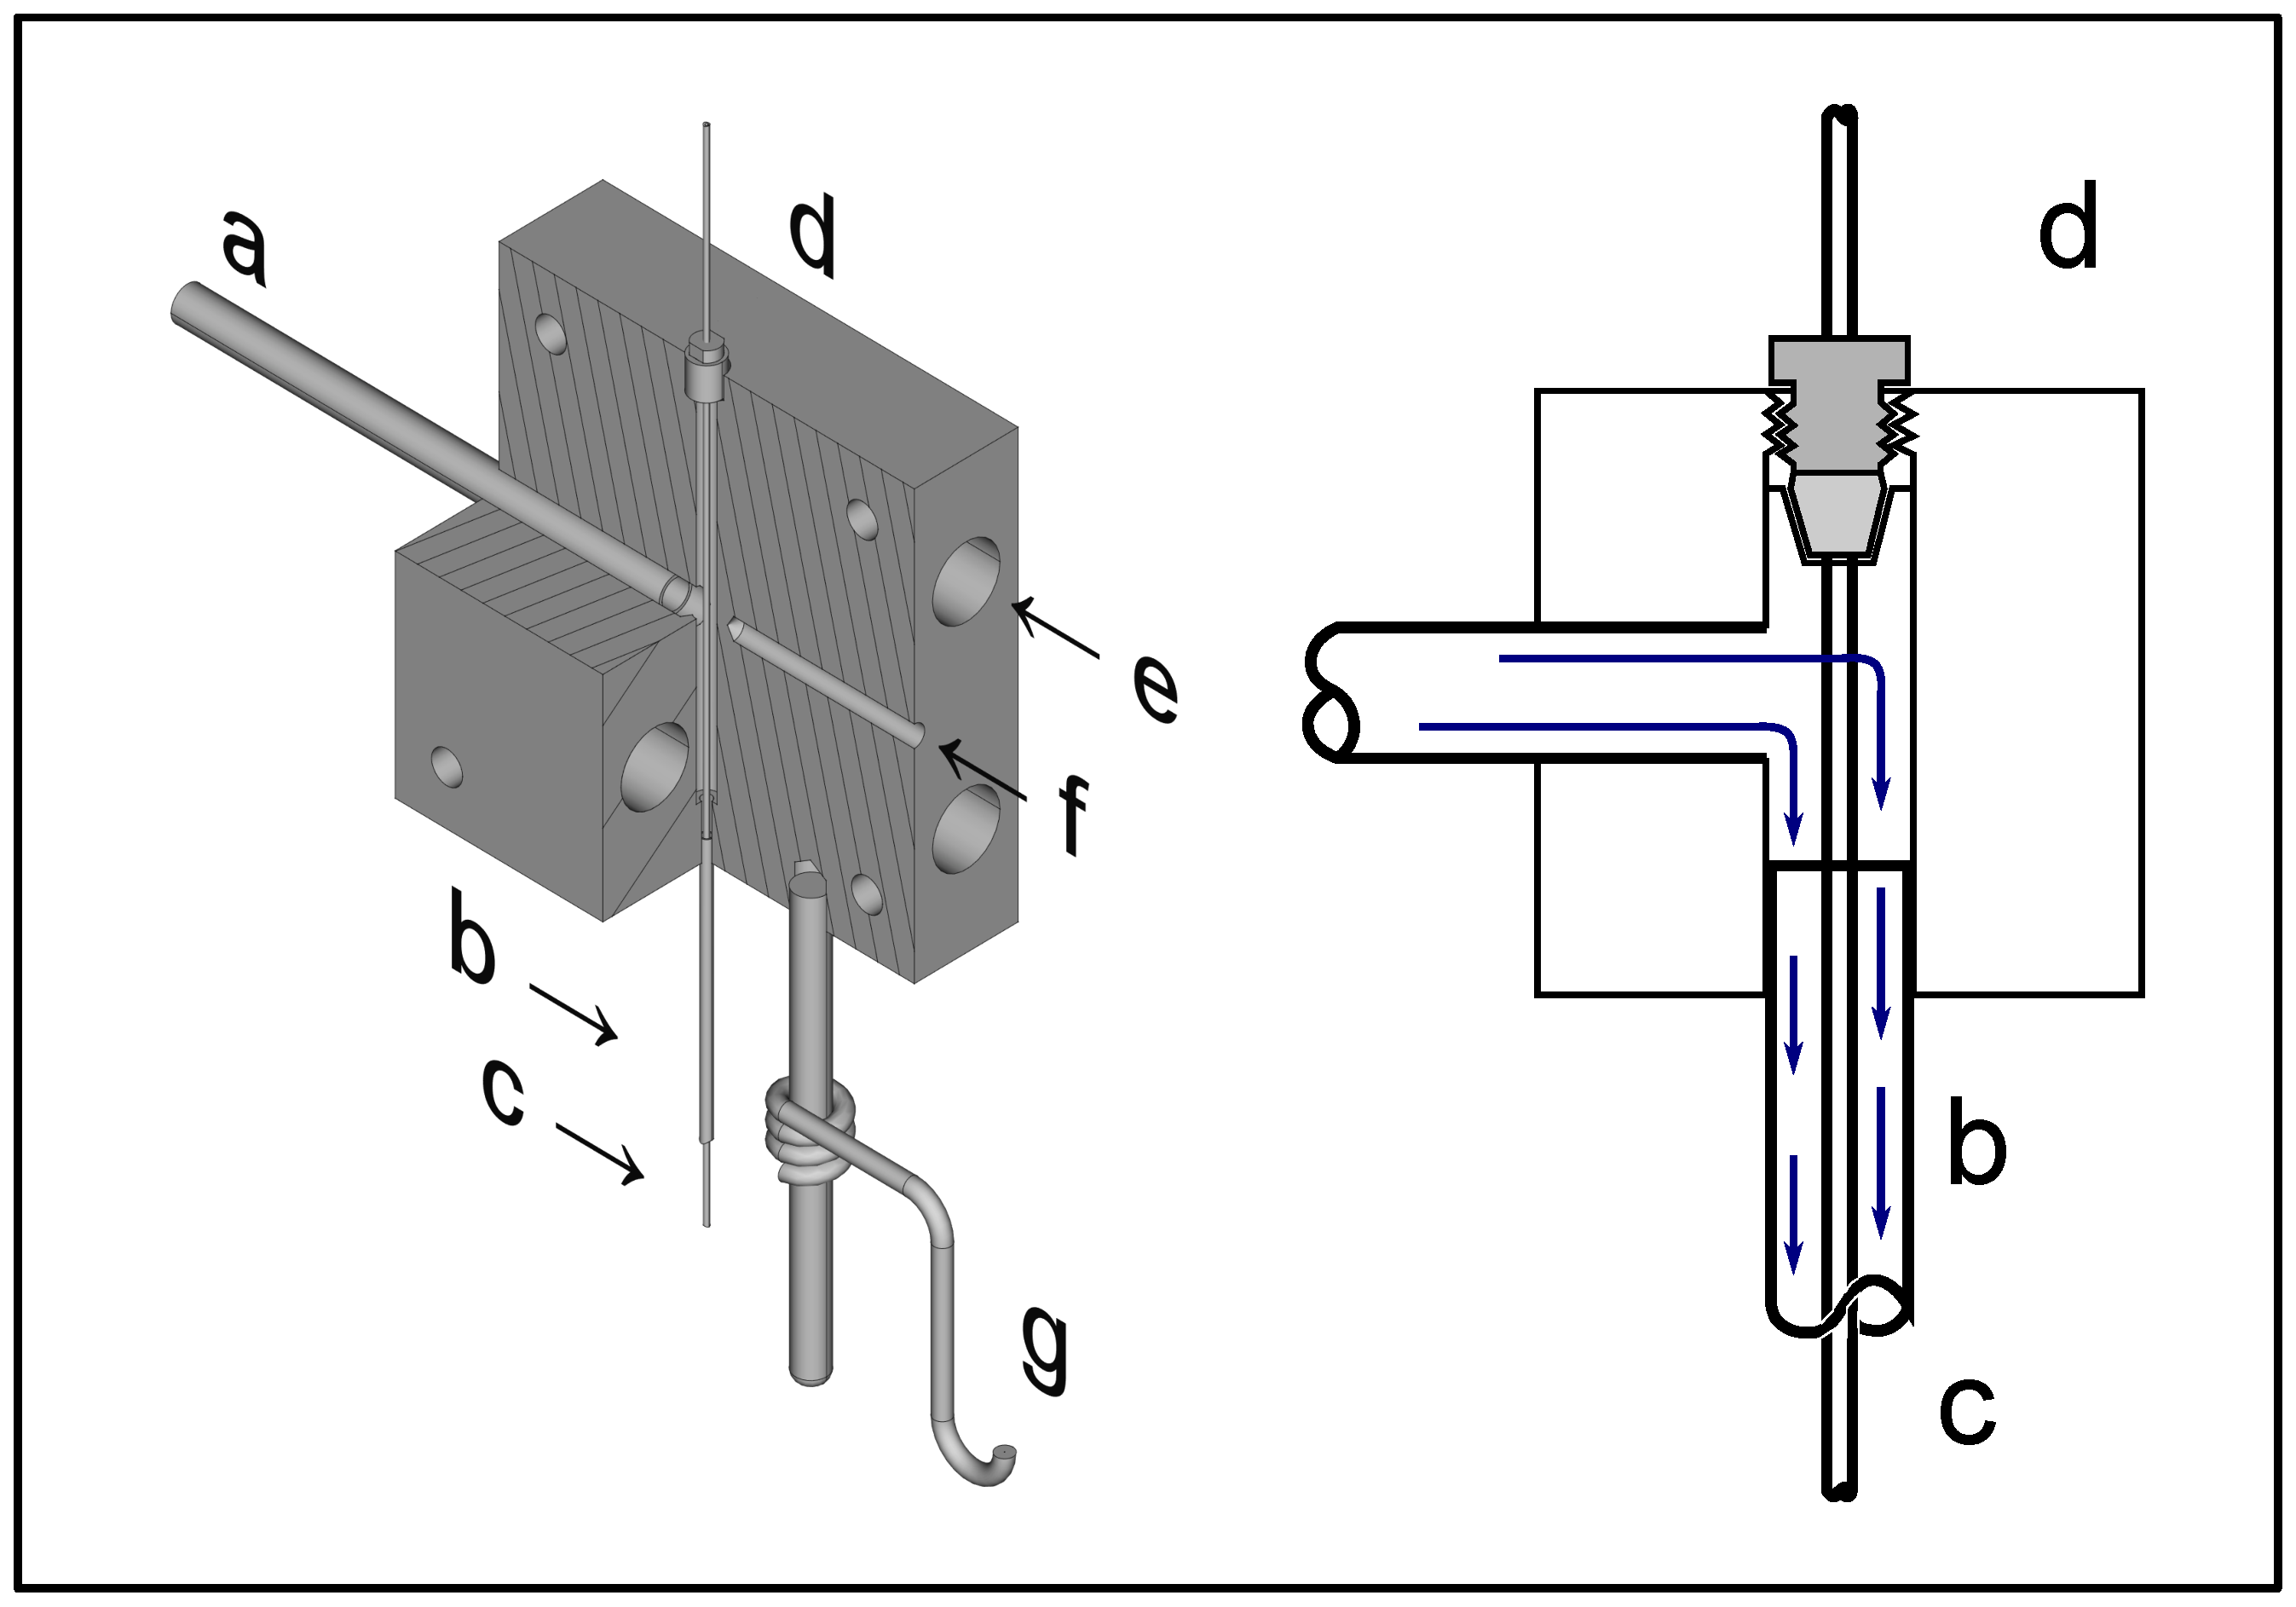
\includegraphics[width=\textwidth]{T-Piece.eps}
	
\caption["The T-piece block"]{Left: A cutaway diagram of the inlet/outlet outlet
T-piece blocks with all the parts to scale, showing (a) the cryogenic coolant
inlet/outlet, (b) the coaxial heater, (c) the capillary column, (d) the
micro-union seal, (e) the cartridge heater socket, (f) the thermocouple socket,
and (g) the connector to which the power feed conductor was soft-soldered.
Right: A schematic diagram showing the flow of the coolant through the T-piece
block into the coaxial heater.}%
	
	\label{fig:Manifold}
\end{figure}
 
The T-piece blocks were mounted on `cars' that slid up and down twin round-bar
rails on brass bushes. The cars carried the weight of the inlet and outlet
T-piece blocks and rigidly aligned the column with the inlet and detector of the
gas chromatograph. The cars were isolated electrically from the rails by a
sandwich construction that included silicone-impregnated mica as insulating material. The
whole of the inlet and outlet T-piece blocks were at the electrical potential of
the coaxial heater ends.

The cryogenic carbon dioxide (Afrox, Tec (Wet)) was supplied from a cylinder
equipped with a dip tube. It flowed to a coil heat exchanger mounted on top of
the Varian GC from where the carbon dioxide flowed down to the cryo shut-off
valve (ASCO, RedHat brand). (The heat exchanger was bathed in a cold
(\SI{-5}{\celsius}) propylene glycol heat transfer fluid.) This arrangement
ensured a supply of liquid CO$_2$ at the shut-off valve, without which some
gaseous CO$_2$ might have to vent through the coaxial heater before the liquid
CO$_2$ coolant could reach it. Downstream of the shut-of valve a 10-turn
metering valve controlled the flow of carbon dioxide into the coaxial heater. At
the outlet end of the coaxial heater the carbon dioxide escaped through the
T-piece block into the atmosphere.

The SFC subsystem consisted of five packed silica columns
(\SI{150}{\milli\metre} × \SI{4.6}{\milli\metre}, \SI{3}{\micro\metre}
particles) (Restek, Pinnacle DB Silica) in series, a sample valve (VICI), and a
stop valve (VICI). Carbon dioxide, (\SI{99.995}{\percent} purity, Air Products)
was supplied to a Varian 8500 piston pump. The inlet pressure of the SFC columns
was controlled by a software proportional controller driving the stepper motor
of the piston pump. The high pressure at the column exit was maintained by a
linear fused silica capillary restrictor with an internal diameter of
\SI{0.050}{\milli\metre}, \SI{800}{\milli\metre} long.

\subsection{Electronics}

The electronics for controlling the fast temperature programmed gas
chromatograph and the SFC front-end was developed in-house. A controlled direct
current was used to heat the coaxial heater. The heating circuit consisted of
the coaxial heater in series with a reference resistor and a ballast resistor.
The reference and ballast resistors were constructed from stainless steel wire
with a diameter of \SI{1.0}{\milli\metre}. The reference resistor had multiple,
parallel conductors, the ballast resistor had a bifilar winding, and both had
air cores. These designs (see Figure \ref{fig:RefRes}) minimized electromagnetic
interference and encouraged heat dissipation. Since the coaxial heater
resistance measurement used a two-wire technique, the current-carrying circuit
was made entirely of soldered joints to minimize stray resistance from
developing in electrical connections.

\begin{figure}
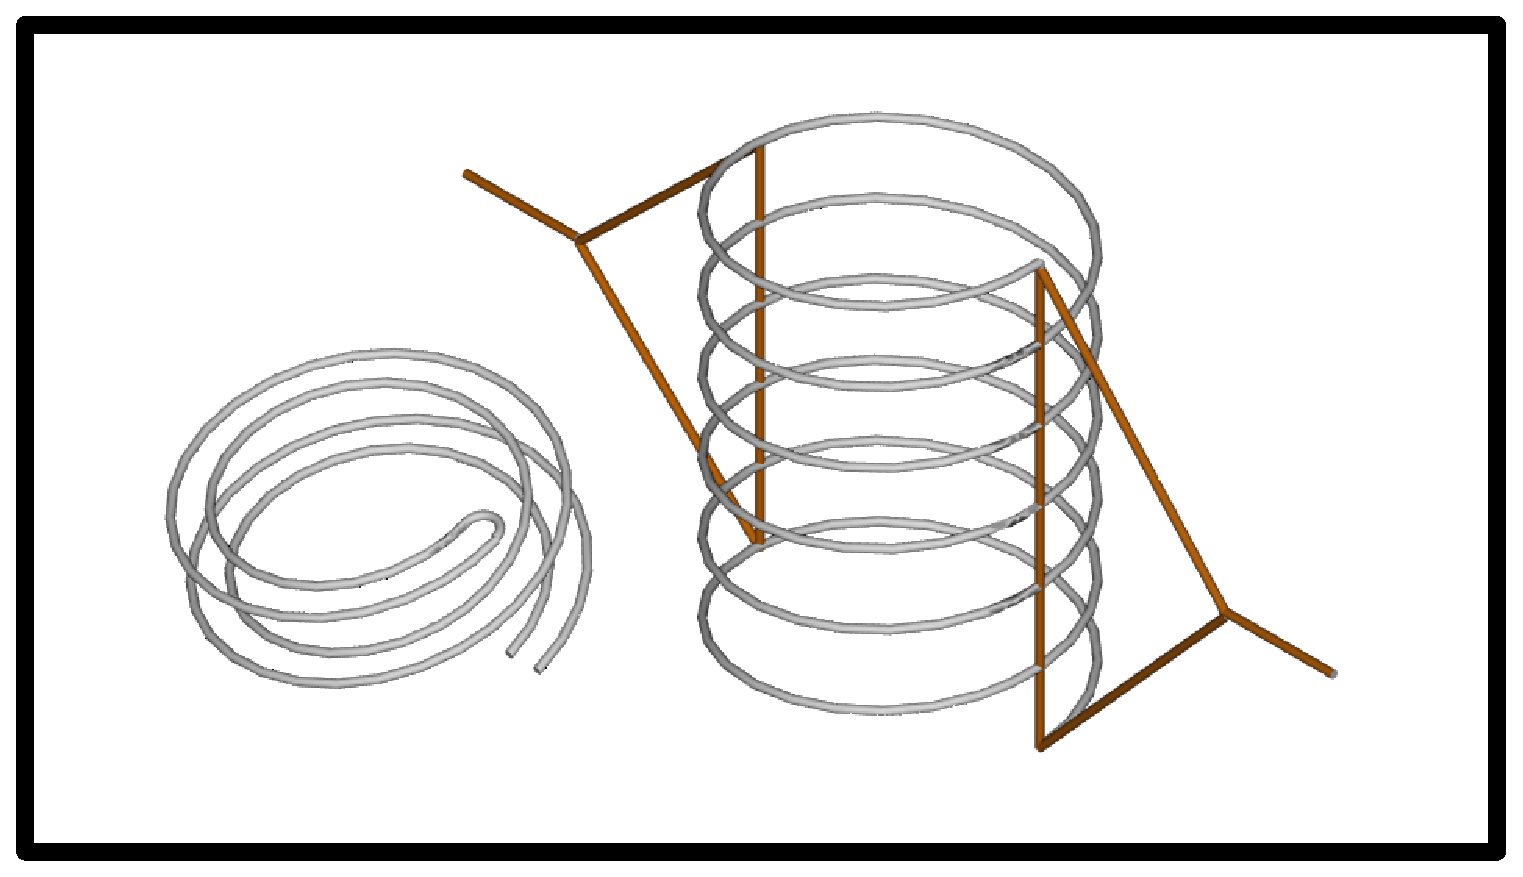
\includegraphics[width=\textwidth]{RefRes.eps}%

\caption{\label{fig:RefRes}An illustration of the designs of the ballast (left)
and reference (right) resistors. The outside diameters of the coils are about
\SI{25}{\milli\metre} and \SI{50}{\milli\metre} respectively. The designs
emphasize heat dissipation by air convection and mitigation of electromagnetic
interference by using parallel conductors.}

\end{figure}

The resistance of the reference resistor ($R_{ref}$) was about \SI{0.005}{\ohm},
the resistance of the coaxial heater ($R_{col}$) was about  \SI{0.3}{\ohm}, and
the resistance of the ballast resistor was about \SI{0.01}{\ohm}, so that most
of the heat in the circuit was dissipated by the coaxial heater.
The potential differences across the coaxial heater ($V_{col}$) and the
reference resistor ($V_{ref}$) were measured (See Figure \ref{fig:Circuit}). If the
resistances of the coaxial heater and the reference resistor were both constant,
the ratio $V_{col}/V_{ref}$ would be constant, independent of the current.
But metals have positive coefficients of resistivity so the resistance of the
coaxial heater will increase with temperature. If the assumption is made that
the temperature of the reference resistor does not change, then the ratio
$V_{col}/V_{ref}$ will be proportional to $R_{col}$. If the resistance $R_{col}$
is assumed to be a monotonically rising function of the temperature ($R_{col} =
f(T)$), then the inverse function will provide the temperature ($T =
f^{-1}(R_{col})$). In practice the voltage $V_{ref}$ is too small to be
digitized directly and needs to be amplified to $V_b$, but it can be shown that
$R_{col}$ is a function of $\left(\frac{dV}{V_b}\right)$, where $dV$ is the
difference between the supply voltage and $V_b$. $dV$ and $V_b$ are of
magnitudes that can be conveniently digitized.

\begin{figure}
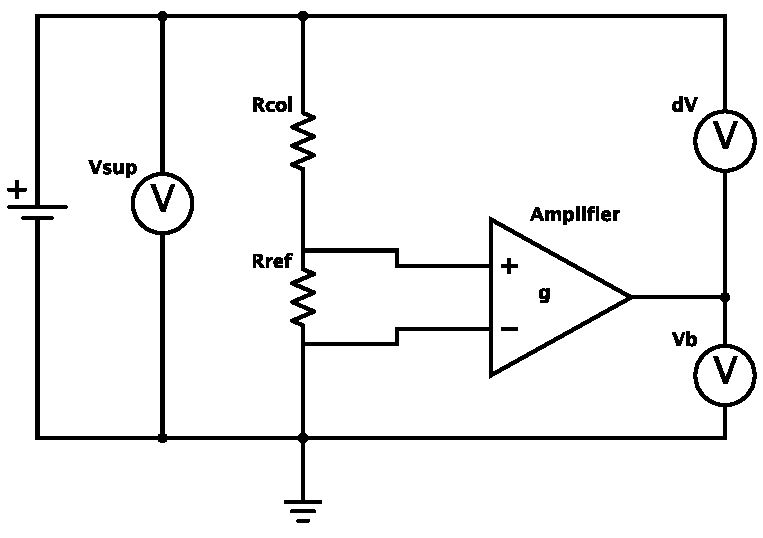
\includegraphics[width=\textwidth]{Column-Heater.pdf}%
\caption{\label{fig:Circuit}A simplified circuit diagram of the resistance measuring circuit.}%
\end{figure}


A bank of six PNP 2N2955 bipolar transistors mounted in parallel on an aluminium
plate air-cooled by two 4-inch fans controlled a current of up to
\SI{20}{\ampere} at \SI{20}{\volt} through the coaxial heater. A two-stage
control system controlled the current. The first stage of the control system was
a PID controller implemented in LabVIEW 7.1\texttrademark{} (National
Instruments). The process variable was the temperature of the coaxial heater, as
calculated from its electrical resistance, and the set value was determined by
the desired chromatographic temperature program. The manipulated variable was
the voltage of the digital-to-analog converter (DAC) of the data
acquisition board. The final stage was an electronic system, where the voltage
applied to the coaxial heater was the process variable, and the set value was a
voltage provided by the DAC. The manipulated variable was the base current of
the power transistors. In summary, the software set a voltage, which set the
power of the coaxial heater. This two-stage design allows for switching of the
control of the coaxial heater from computer control to manual control by a
potentiometer on the instrument front panel. Being able to control the power of
the coaxial heater manually is extremely useful during development and
fault-finding.

AD595 monolithic thermocouple amplifiers (Analog Devices) with integral cold
junction compensation were used to condition the signal of the K-type
thermocouples that were used for temperature monitoring and calibration. Solid
state relays (Opto 22, Model 240D3) were used to switch the inlet and outlet
T-piece block cartridge heaters (described above) on and off. Pulse width
modulation, implemented in software, was used to control the amount of heat
produced by the cartridge heaters, and hence the temperature of the T-piece
blocks. A PCI-6014 multifunction data acquisition board (National
Instruments\texttrademark{}) was used to interface the electronics with the
computer.

\subsection{Coaxial heater temperature calibration}

The temperature of the coaxial heater was calibrated by constructing a
thermocouple probe from \SI{0.025}{\milli\metre} diameter thermocouple alloy
wire (T1 and T2 alloys, Goodfellow) threaded inside a \SI{1000}{\milli\metre}
length of \SI{0.25}{\milli\metre} i.d. fused silica capillary. This thermocouple
probe was then threaded inside the coaxial heater (just like the capillary
column during GC operation) to record the temperature of the heater. The
recorded temperature could then be used to calibrate the coaxial heater
resistance.

\subsection{Heating uniformity}

To determine whether the coaxial heater was heating the column with acceptable
uniformity, we used two methods. Firstly, we acquired thermographic videos of
the coaxial heater, using a FLIR T660 infrared camera. Secondly, for experiments
in determining temperature gradients, a thermocouple probe was constructed as
described above, except that the probe contained two thermocouples,
\SI{330}{\milli\metre} apart, equidistant from the ends.

\subsection{Software}

\subsubsection{Instrument Control}
The software for controlling the instrument and collecting data was written in
LabVIEW. Two main loops were used. One controlled the various aspects of the
instrument, in particular the temperature control, and ran with a period of
\SI{200}{\milli\second}. The second main loop collected the data and ran as
often as the hardware allowed.

% The multi-threading capabilities of LabVIEW greatly eased development. Each
% subsystem of the instrument was controlled by a separate loop, allowing it to
% run at its own rate. In particular, running the manifold heater controls and
% pressure control as separate threads from the chromatography control and data
% loops simplified development.

The coaxial heater temperature was controlled by
proportional-integral-derivative (PID) controllers implemented in LabVIEW. In
practice it was found that only proportional and integral control was needed.
We used a privately published\cite{Peacock2008} step-by-step implementation of
the Cohen-Coon loop tuning method. Subsidiary PID controllers controlled the
T-piece block temperatures and the CO$_2$ pump pressure.

%The version of LabVIEW used did not have any real-time capability, so timings are approximate and indeterminate, but good enough for chromatography. 

\subsubsection{Data structure}
In GC×GC, 2D data is recorded as a continuous detector output stream, as if it
were a 1D GC chromatogram, and later converted into a 2D chromatogram, using
knowledge of the modulation period. For two reasons we could not use this
approach. Firstly, in our instrument the first (SFC) dimension runs in a
stop-flow mode making continuous data recording inappropriate. Secondly, the
duration of the cooling cycle can vary slightly, which could introduce
unacceptable variation in \textsuperscript{2}D retention times. We therefore
started detector output recording at the start of each GC fast temperature
program, using the GC start time as the elution time of the first (SFC)
dimension.

\subsubsection{Data visualization}
For data visualization we used the technical computing system Mathematica
11.3\texttrademark{} (Wolfram).  The collected data was first converted to a
list of three-element lists, with $^1$D retention time, $^2$D retention time,
and detector signal as the elements of the inner lists. The Mathematica
functions \texttt{List3DPlot[]} and \texttt{ContourPlot[]} was then used to
plot 3D chromatograms or contour plots respectively.

\section{Results and Discussion}

\subsection{Heating uniformity}

As a first step in developing the coaxial heater, we tried to answer the
question about its temperature uniformity. Because the temperature coefficient
of resistivity of metals is positive, in the absence of equalizing heat flow
along the length of conductor the resistive heating process in a long, thin tube
is inherently unstable. To monitor the temperature profile along its length we
acquired a thermographic video of the coaxial heater (See Supplementary Online
Material). The video shows that the coaxial heater heats and cools smoothly with
no run-away hot spots. A still image from the video is show in Figure
\ref{fig:ThermImg}.

%Modeling the coaxial heater thermo-electrically might be a fruitful exercise.

\begin{figure}
  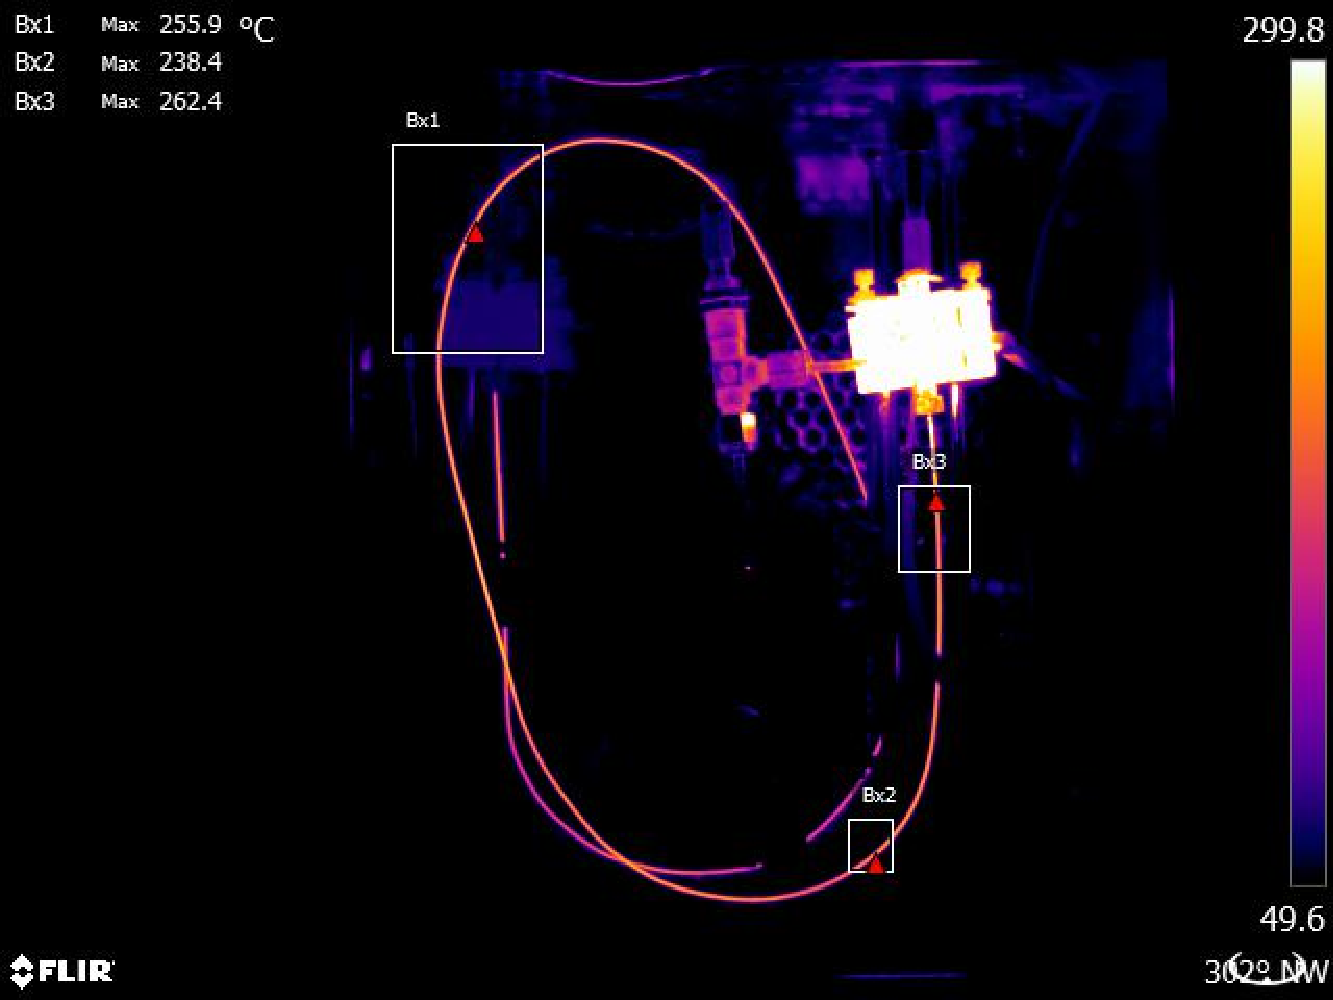
\includegraphics[width=\textwidth]{1-16.pdf}%
  \caption{\label{fig:ThermImg} A frame from the thermographic video of the coaxial heater. There are no evident run-away hot spots.}%
\end{figure}

To quantify the non-uniformity of the coaxial heater, a dual thermocouple probe
was inserted into the coaxial heater. The two thermocouples in the probe were
\SI{330}{\milli\metre} apart and positioned in the central third of the coaxial
heater. The coaxial heater was submitted to a repeated program of cooling and
ballistic heating. The recorded data (see Figure \ref{fig:Repeatability}) shows
that the two thermocouples reported different temperatures and that the
difference changed during the heating, implying that the coaxial heater did not
cool or heat perfectly uniformly. But the temperature differences between the
two points were small (approximately \SI{10}{\celsius} at most), stable, and
repeatable and should not prevent good chromatography. In fact, a small
longitudinal gradient, with the lower temperature nearer the detector, will
produce sharper peaks\cite{Contreras2013}. These data also show that ballistic
heating is not repeatable enough for gas chromatography, as can be seen in the
variation in temperatures at the end of the heating runs.

\begin{figure}
  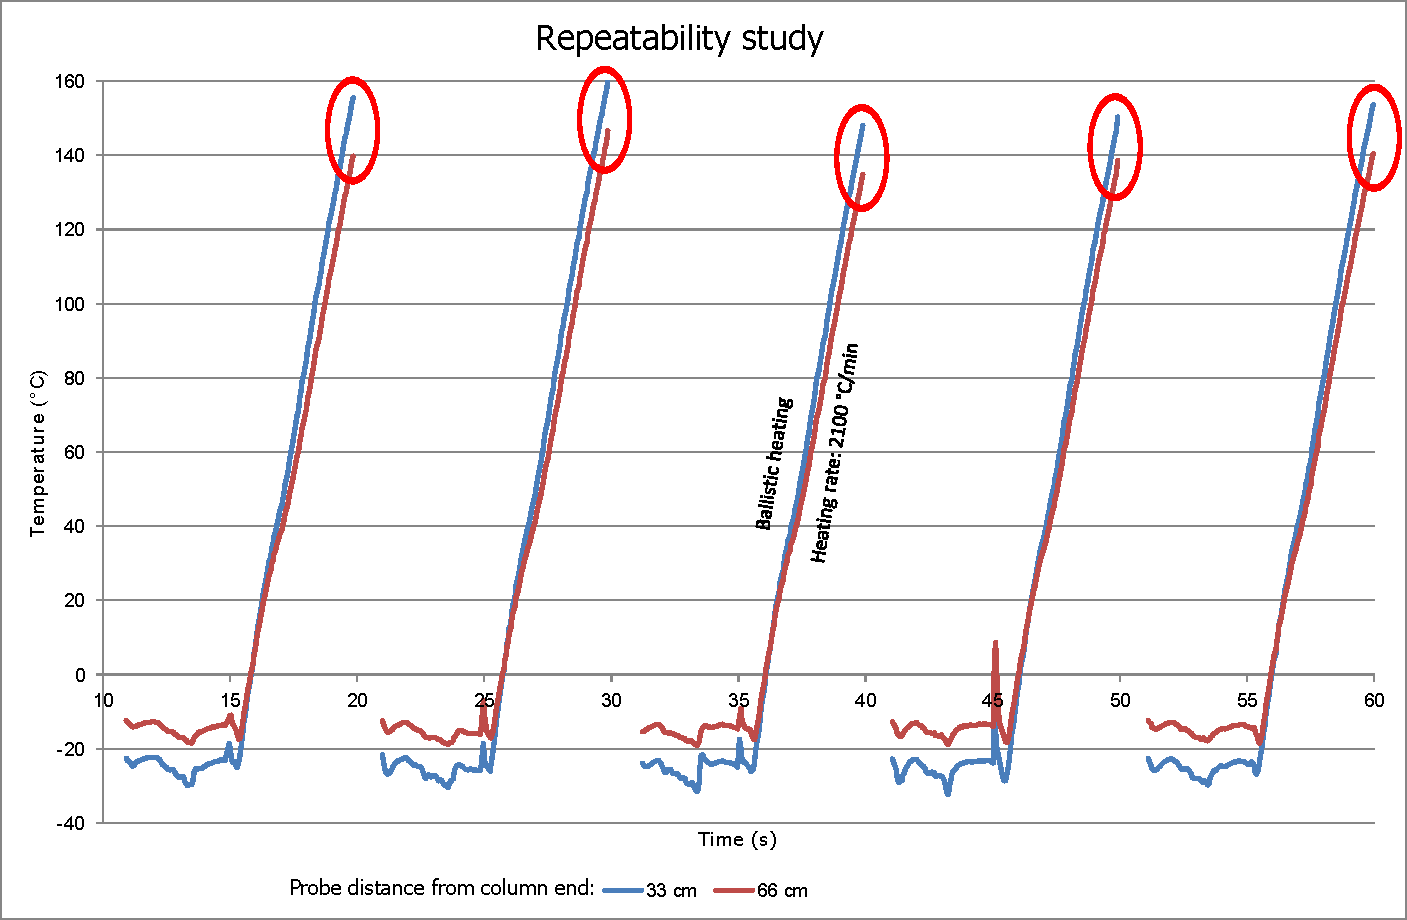
\includegraphics[width=\textwidth]{cp.pdf}%
  
  \caption{\label{fig:Repeatability} The temperature difference between two
  points in the coaxial heater. The temperature difference established during
  cooling is reversed during heating, which shows that gradients exist, but they
  are small and repeatable.}

\end{figure}

\subsection{Temperature calibration}

While it is conceptually possible to have a fast temperature program by using
the voltage/current ratio alone as a temperature indicator and controlled
variable, it would be hard to design chromatographic methods or translate
methods without a knowledge of the real temperature. Therefore, we went to some
effort to calibrate the coaxial heater.

To calibrate a thermometer, the thermometer under test and its calibration
environment must be in equilibrium. This requirement is hard to meet in our
calibration, because a single point (the junction of the thermocouple) needs to
be in equilibrium with the length of the coaxial heater during the full fast
heating cycle. This equilibrium would be very difficult to maintain, especially
because the uniformity of heating cannot be guaranteed, and is additionally
influenced by the presence of the hot T-piece blocks --- for a totally uniform
heating of the coaxial heater the T-piece blocks would have to be at the same
temperature as the coaxial heater. Acknowledging these limitations, we performed
a calibration procedure assuming that the thermocouple junction was in
equilibrium with the coaxial heater, which was assumed to be of uniform
temperature over its length. Because these assumptions are simplifications, or
for other overlooked reasons, the calibration curve (see Figure
\ref{fig:TempCal}) is oddly curved, and we arbitrarily fitted a B-spline to the
data points. This procedure can be automated\cite{Zheng2012}. Points from this
B-spline curve were then extracted to create a calibration curve, from which an
estimate of the temperature can be calculated by linear
interpolation\cite{Possolo2017}.

\begin{figure}
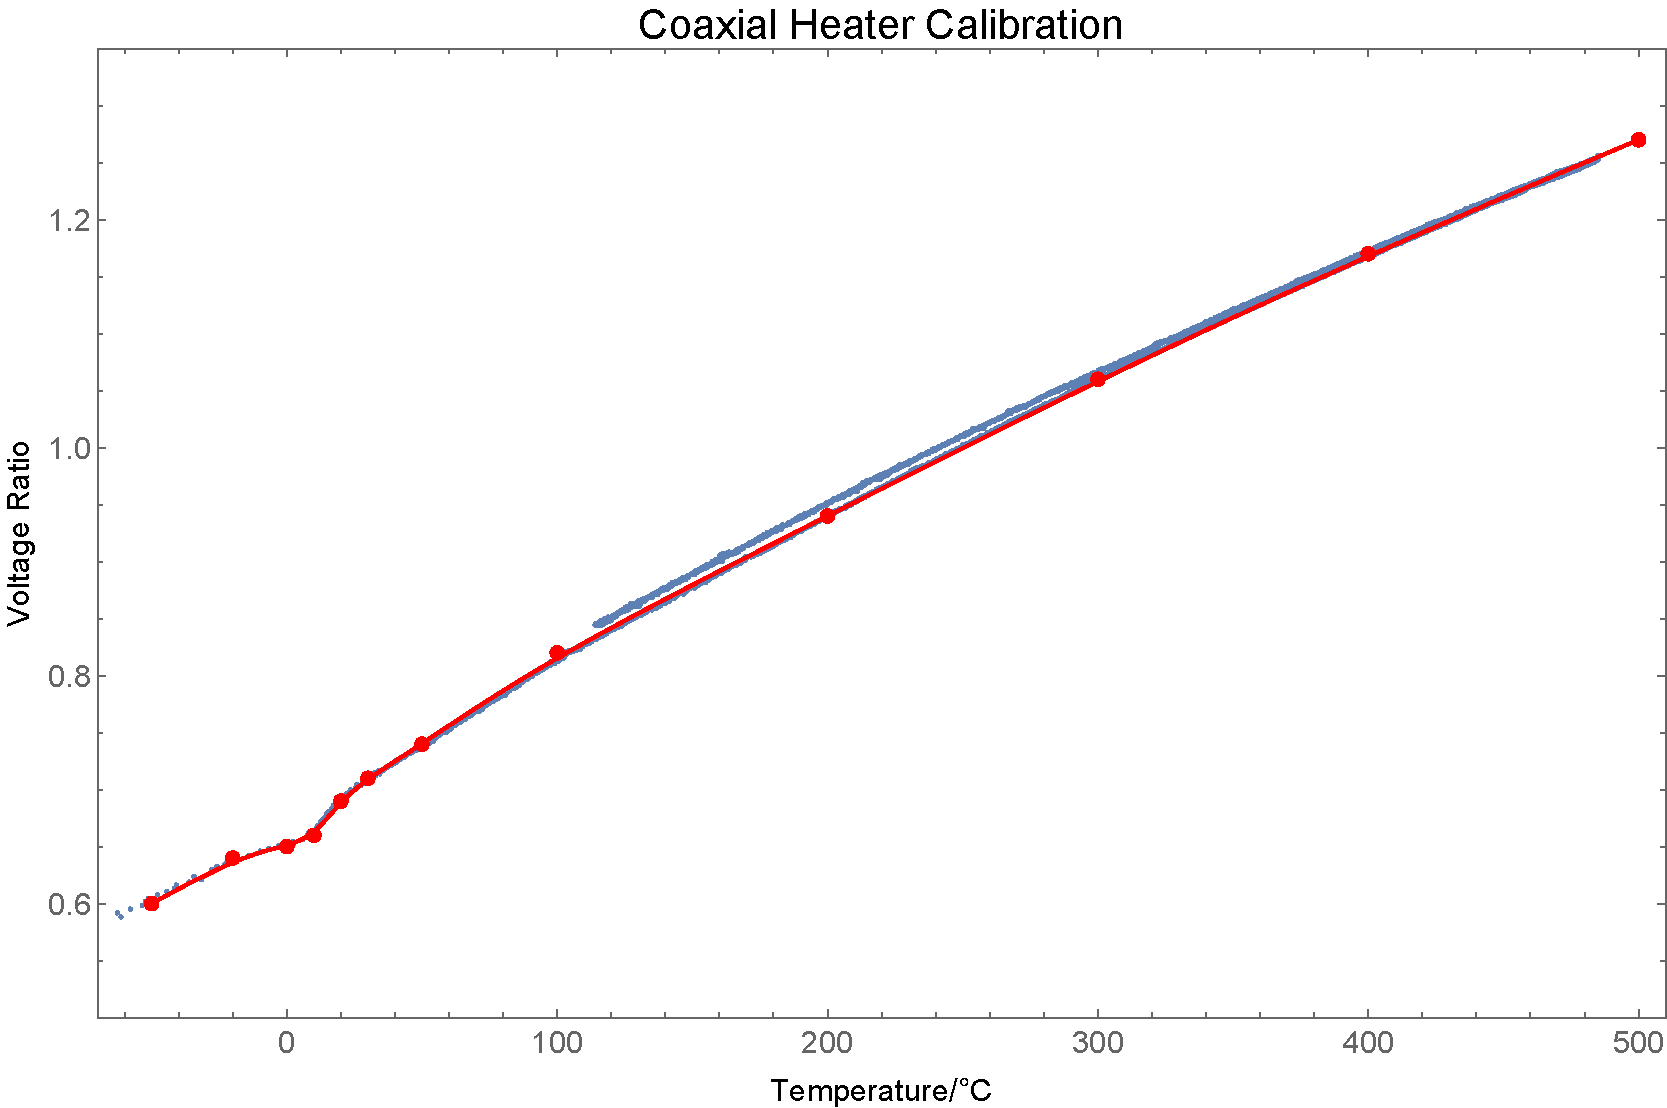
\includegraphics[width=\textwidth]{2019_07_12_B-spline_fit_CPlot.pdf}%

\caption{\label{fig:TempCal}A calibration curve of the coaxial heater. The blue
points represent the experimental data, and the red line is a B-spline fitted
manually to the data. The red markers are points extracted from the B-spline.
The temperature is obtained by linear interpolation between markers.}%

\end{figure}

\subsection{Heating rate}

To achieve good resolution in temperature-programmed chromatography, a good rule
of thumb for the heating rate is \SI{10}{\celsius} per void
time\cite{Blumberg2000}. With hydrogen as carrier gas in a
\SI{0.25}{\milli\metre} i.d. column the efficiency-optimized linear velocity is
\SI{40}{\centi\metre\per\second}. Then the void time of a \SI{1}{\metre} column
is \SI{2.5}{\second}, so the recommended heating rate is \SI{10}{\celsius} per
\SI{2.5}{\s}, which is \SI{4}{\celsius\per\second}, or
\SI{240}{\celsius\per\minute}. Since in fast chromatography excess peak
resolution is traded for shorter run times, higher-than-optimum flow rates will
be used, so higher heating rates will be required. For narrower columns the flow
will be even higher so that heating rates of more than
\SI{1000}{\celsius\per\minute} will be required.

The attainable heating rate is a function of power to the heater and of the
temperature required. (In the instrument presented here the power was limited by
the voltage output range of the DAC of the data acquisition board, and not by
the power of the heater.) We were able to maintain controlled heating rates of
\SI{2500}{\celsius\per\minute} up to \SI{400}{\celsius}, or up to \SI{4000}{\celsius\per\minute}
up to \SI{350}{\celsius} (See Figure \ref{fig:MaxHeatingRate}). The heating
rates attainable seem to be high enough for the most demanding fast gas
chromatography.

\begin{figure}
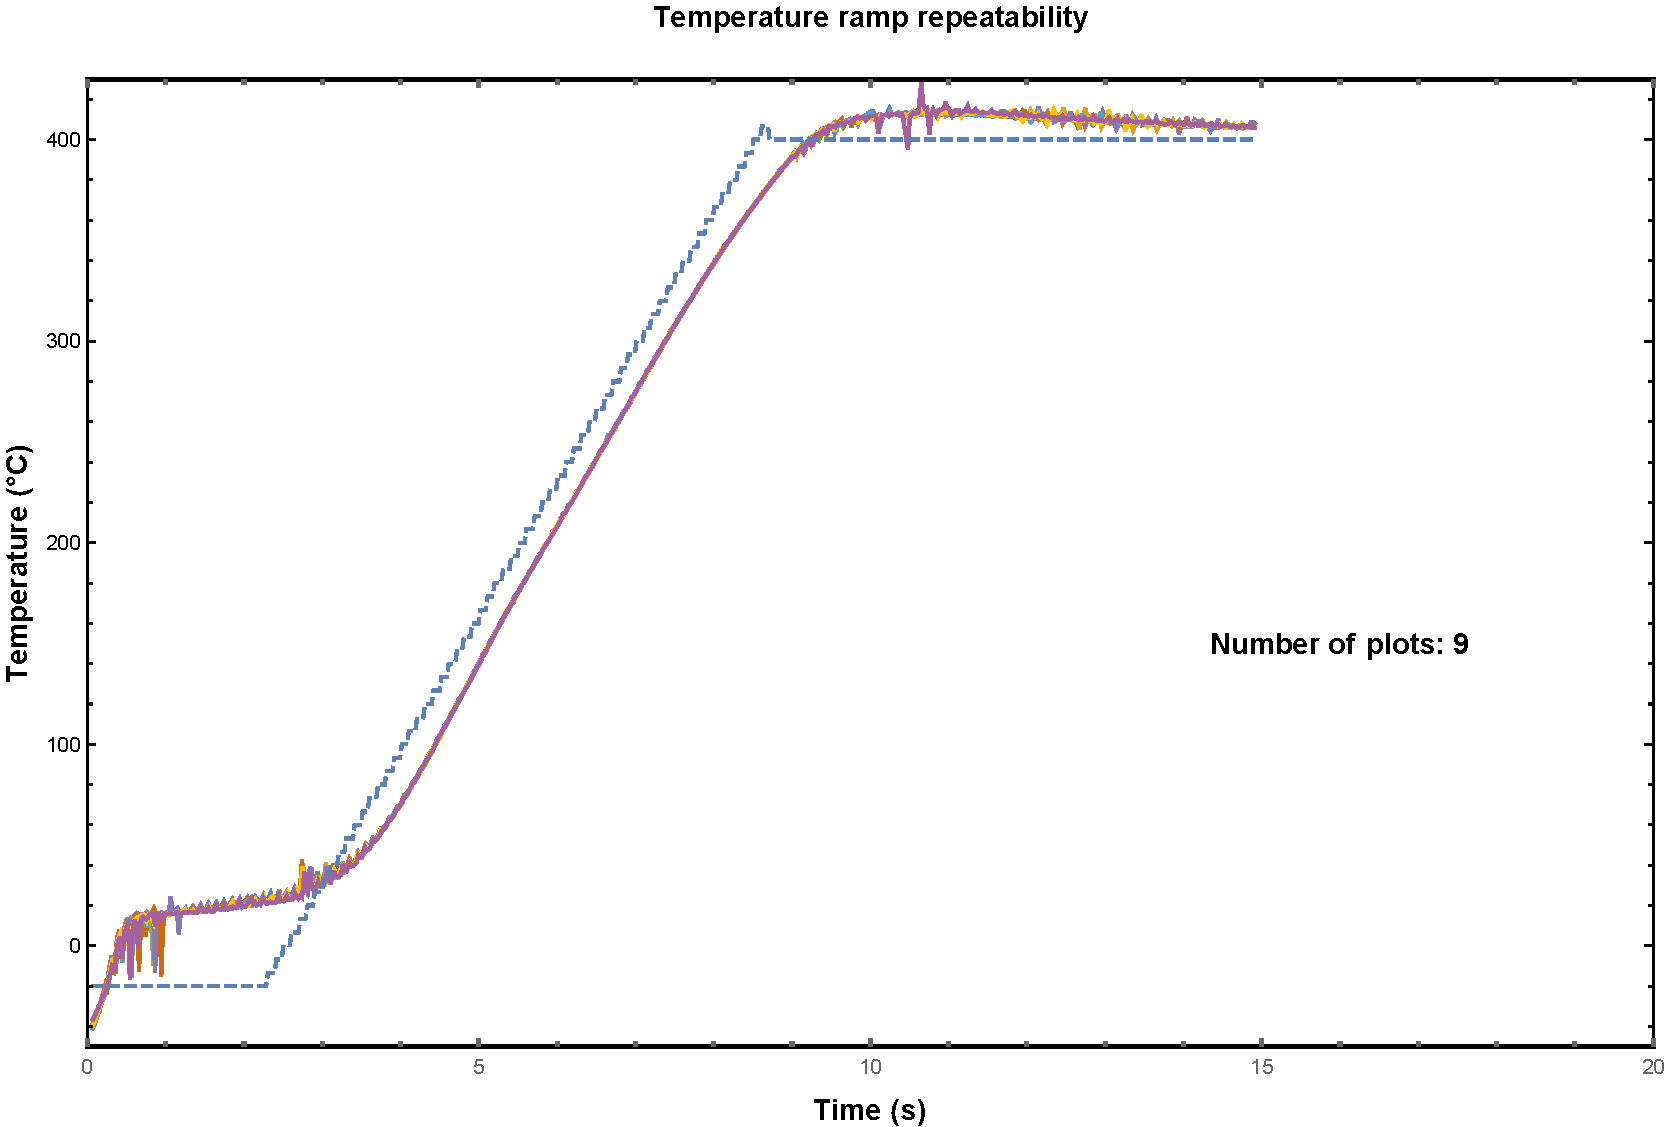
\includegraphics[width=\textwidth]{high_rate_heating.pdf}%

\caption{\label{fig:MaxHeatingRate}A graph of \num{9} identical, consecutive
temperature ramps overlaid. The heating rate is \SI{4000}{\celsius\per\minute}.
The temperature follows the setpoint faithfully up to \SI{350}{\celsius}}

\end{figure}

\subsection{Cooling rate}

Using evaporating carbon dioxide as a powerful coolant, it was possible to cool
down the column at a rate of \SI{5100}{\celsius\per\minute}. The cooling rate
depends on the setting of the metering valve, with the lowest coaxial heater
temperatures and smallest gradients achieved at an intermediate flow of about
\SI{30}{\gram\per\minute}.

%At high flows the coaxial heater fills with liquid carbon dioxide, with
%evaporation taking place only at the outlet end. At low flow, evaporation takes
%place only at the inlet end, the rest of the coaxial heater being filled with
%gaseous carbon dioxide. This was easily deduced by observing the layer of frost
%from atmospheric water forming on the coaxial heater. Under ideal conditions the
%frost would form a continuous layer on the outside of the coaxial heater, which
%also gave the lowest temperature and best cooling rate.

\subsection{Repeatability}

Comprehensive two-dimensional chromatography depends heavily on repeatable
\textsuperscript{2}D separations. To test for chromatographic repeatability, we
added small amounts of hydrocarbons to the \textsuperscript{1}D mobile phase.
They are unretained on the silica stationary phase and are therefore present in
every fraction of the SFC eluate in equal amounts and should yield identical
\textsuperscript{2}D chromatograms. Results obtained from creating a 2D blank
chromatogram with two alkanes in the mobile phase are summarized in Table
\ref{tab:table1}. The peak widths were about \SI{500}{\milli\second}, so the
\SI{20}{\milli\second} standard deviation for hexadecane means that the
variation in retention time is only about \SI{10}{\percent} of the peak width.
The relative standard deviations (RSD) of retention times were similar to those
obtained in GC×GC\cite{Shellie2002}.

\begin{table}

\caption{\label{tab:table1}A summary of retention time repeatability of alkanes
separated on the fast temperature programmed chromatograph.}

\begin{ruledtabular}
\begin{tabular}{lllll}
Compound & n & t\textsubscript{r} (s) & S.D. of t\textsubscript{r} (s)& R.S.D. of t\textsubscript{r} (\%)\\
\hline
Dodecane & 73 & 5.07 & 0.023 & 0.46\\
Hexadecane & 73 & 6.58 & 0.052 & 0.78\\
\end{tabular}
\end{ruledtabular}
\end{table}

\subsection{Chromatography}

Comprehensive two-dimensional chromatography is made possible by having different
retention mechanisms in the columns of the two dimensions. When fatty acid
methyl esters (FAMEs) are chromatographically separated on bare silica with neat
carbon dioxide as a mobile phase, they are separated according to the number of
double bonds, independent of chain length\cite{Smith2001}. On a GC column, FAMEs
are separated according to volatility or, equivalently, chain length. Therefore,
when SFC and GC are comprehensively coupled, we can expect FAMEs to have a
highly orthogonal separation.

We prepared FAMEs by esterifying oil samples, following an official
method\cite{AOCS2017}. Of these samples, \SI{0.2}{\micro\litre} was injected
into the pure carbon dioxide mobile phase at \SI{200}{\bar} and room temperature
and eluted through bare silica. We collected \SI{10}{\second} fractions of SFC
eluate on the cold GC column. The fast temperature program ramped the GC column
temperature from \SI{-20}{\celsius} to \SI{350}{\celsius} in \SI{10}{s}
(\SI{2200}{\celsius\per\second}), then maintaining \SI{350}{\celsius} for
\SI{2}{\second}. Then the cooling system would activate and cool the column to
\SI{-20}{\celsius} or below, ready to trap the next SFC fraction. In this way a
series of GC chromatograms of SFC fractions were recorded to build up a 2D
chromatogram. Figure \ref{fig:2DChromatogram} shows a 2D chromatogram of a
sample of FAME prepared from canola oil. This 2D chromatogram consists of
\num{132} fast GC chromatograms collected in approximately \SI{90}{\minute}.

\begin{figure}
  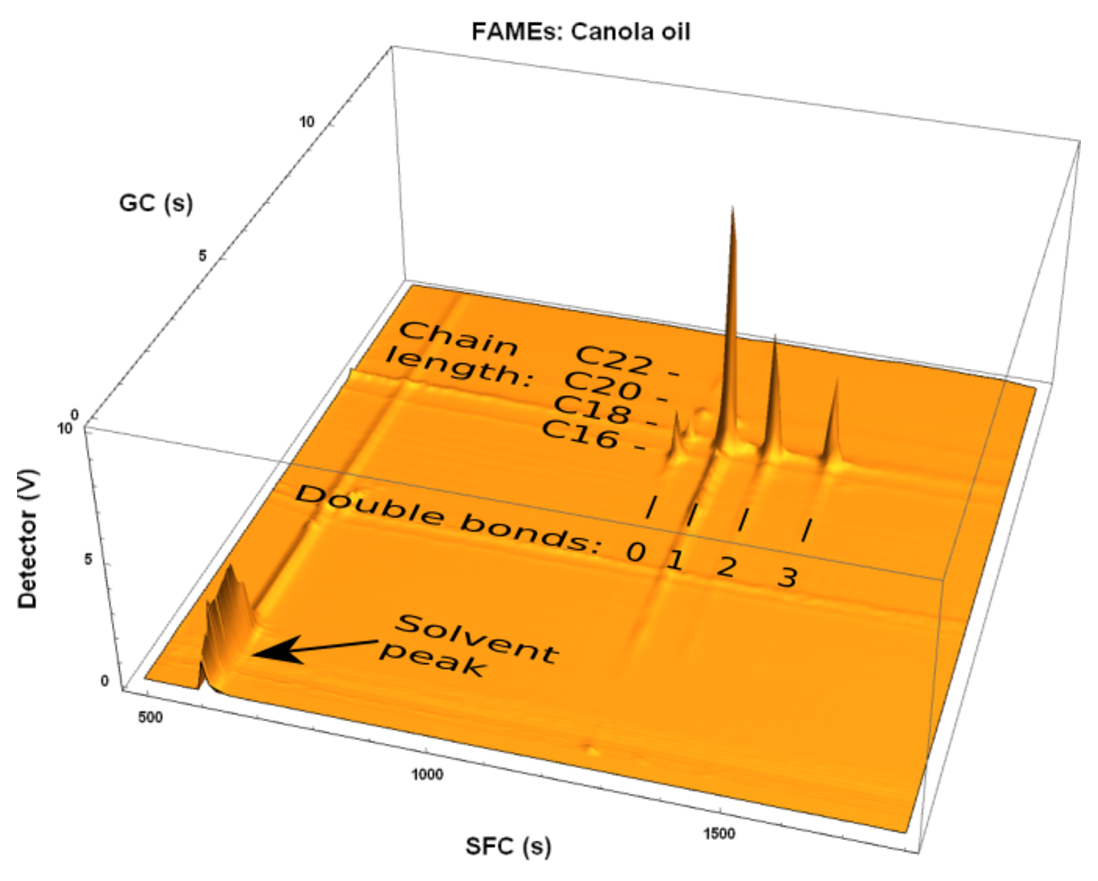
\includegraphics[width=\textwidth]{Interpretation.eps}

\caption{\label{fig:2DChromatogram}A 2D chromatogram of FAMEs derived from
canola oil. It is clear that the oil consists mostly of unsaturated fatty
acids.}

\end{figure}

\section{Conclusion}

To our knowledge, the cycle time of this new temperature programmed GC is
unmatched in the literature, and it allows for the improved performance of
SFC×GC instruments. The fast GC will be of interest to all GC analyses of
highly dynamic chemical systems, including on-line monitoring and control of
fast laboratory or industrial reactions.

The low thermal mass of the heater and column simplifies heating and cooling of
a portable fast GC, reducing electrical and carbon dioxide coolant requirements.
When sub-ambient temperatures and extreme cycle times are not essential,
compressed air could also serve to cool the column.

% If in two-column mode, this environment will change to single-column format so that long equations can be displayed. 
% Use only when necessary.
%\begin{widetext}
%$$\mbox{put long equation here}$$
%\end{widetext}

% Figures should be put into the text as floats. 
% Use the graphics or graphicx packages (distributed with LaTeX2e). EPSFig is no longer fully supported.
% See the LaTeX Graphics Companion by Michel Goosens, Sebastian Rahtz, and Frank Mittelbach for examples. 
%
% Here is an example of the general form of a figure:
% Fill in the caption in the braces of the \caption{} command. 
% Put the label that you will use with \ref{} command in the braces of the \label{} command.
%
% \begin{figure}
% \includegraphics{}% % Important NOTE: Please make certain your figures do not include local directory paths. ex. "c:\file\sub\fig1.eps"
% \caption{\label{}}%
% \end{figure}

% Tables may be be put in the text as floats.
% Here is an example of the general form of a table:
% Fill in the caption in the braces of the \caption{} command. Put the label
% that you will use with \ref{} command in the braces of the \label{} command.
% Insert the column specifiers (l, r, c, d, etc.) in the empty braces of the
% \begin{tabular}{} command.
%
% \begin{table}
% \caption{\label{} }
% \begin{tabular}{}
% \end{tabular}
% \end{table}

\section*{Supplementary Material}

In the supplementary material we provide a thermographic video of the coaxial
heater heating and cooling, which demonstrates the even of heating of the
coaxial heater and its rapid cooling by evaporating carbon dioxide.

% If you have acknowledgments, this puts in the proper section head.

\begin{acknowledgments}
%Put your acknowledgments here.

Prof. Walter Meyer of the Department of Physics at the University of Pretoria
supplied the idea for the resistance-measuring electronic circuit. Nico van
Vuuren machined the T-piece blocks and their mounting rails. We thank Restek for
the generous donation of the packed silica columns. Reinhardt Heymans from FLIR
Systems recorded the thermographic videos at no cost. David Masemula kept the
laboratory supplied with consumables.

\end{acknowledgments}

% Create the reference section using BibTeX:
%\bibliography{RSI-2019_05}
% Run this once to generate your BBL file. Then copy the contents of your BBL file into your main latex file, commenting out "\bibliography"

%%%%%%%%%%%%%%%%%%%%%%%%%%%%%%%%%%%%%%%%%%%%%%%%%%%%%%%%
% BBL file contents start
%aipnum4-2.bst 2019-01-14 (MD) hand-edited version of apsrev4-1.bst
%Control: key (0)
%Control: author (8) initials jnrlst
%Control: editor formatted (1) identically to author
%Control: production of article title (0) allowed
%Control: page (1) range
%Control: year (1) truncated
%Control: production of eprint (0) enabled
\begin{thebibliography}{35}%
\makeatletter
\providecommand \@ifxundefined [1]{%
 \@ifx{#1\undefined}
}%
\providecommand \@ifnum [1]{%
 \ifnum #1\expandafter \@firstoftwo
 \else \expandafter \@secondoftwo
 \fi
}%
\providecommand \@ifx [1]{%
 \ifx #1\expandafter \@firstoftwo
 \else \expandafter \@secondoftwo
 \fi
}%
\providecommand \natexlab [1]{#1}%
\providecommand \enquote  [1]{``#1''}%
\providecommand \bibnamefont  [1]{#1}%
\providecommand \bibfnamefont [1]{#1}%
\providecommand \citenamefont [1]{#1}%
\providecommand \href@noop [0]{\@secondoftwo}%
\providecommand \href [0]{\begingroup \@sanitize@url \@href}%
\providecommand \@href[1]{\@@startlink{#1}\@@href}%
\providecommand \@@href[1]{\endgroup#1\@@endlink}%
\providecommand \@sanitize@url [0]{\catcode `\\12\catcode `\$12\catcode
  `\&12\catcode `\#12\catcode `\^12\catcode `\_12\catcode `\%12\relax}%
\providecommand \@@startlink[1]{}%
\providecommand \@@endlink[0]{}%
\providecommand \url  [0]{\begingroup\@sanitize@url \@url }%
\providecommand \@url [1]{\endgroup\@href {#1}{\urlprefix }}%
\providecommand \urlprefix  [0]{URL }%
\providecommand \Eprint [0]{\href }%
\providecommand \doibase [0]{https://doi.org/}%
\providecommand \selectlanguage [0]{\@gobble}%
\providecommand \bibinfo  [0]{\@secondoftwo}%
\providecommand \bibfield  [0]{\@secondoftwo}%
\providecommand \translation [1]{[#1]}%
\providecommand \BibitemOpen [0]{}%
\providecommand \bibitemStop [0]{}%
\providecommand \bibitemNoStop [0]{.\EOS\space}%
\providecommand \EOS [0]{\spacefactor3000\relax}%
\providecommand \BibitemShut  [1]{\csname bibitem#1\endcsname}%
\let\auto@bib@innerbib\@empty
%</preamble>
\bibitem [{\citenamefont {Watson}, \citenamefont {Horton},\ and\ \citenamefont
  {Staples}(1991)}]{Watson1991}%
  \BibitemOpen
  \bibfield  {author} {\bibinfo {author} {\bibfnamefont {G.}~\bibnamefont
  {Watson}}, \bibinfo {author} {\bibfnamefont {W.}~\bibnamefont {Horton}},\
  and\ \bibinfo {author} {\bibfnamefont {E.}~\bibnamefont {Staples}},\
  }\bibfield  {title} {\enquote {\bibinfo {title} {Gas chromatography utilizing
  saw sensors},}\ }in\ \href {https://doi.org/10.1109/ULTSYM.1991.234175}
  {\emph {\bibinfo {booktitle} {IEEE 1991 Ultrasonics Symposium,}}},\
  Vol.~\bibinfo {volume} {1}\ (\bibinfo {year} {1991})\ pp.\ \bibinfo {pages}
  {305--309}\BibitemShut {NoStop}%
\bibitem [{\citenamefont {He}, \citenamefont {Liu},\ and\ \citenamefont
  {Liu}(2014)}]{He2014}%
  \BibitemOpen
  \bibfield  {author} {\bibinfo {author} {\bibfnamefont {S.}~\bibnamefont
  {He}}, \bibinfo {author} {\bibfnamefont {J.}~\bibnamefont {Liu}},\ and\
  \bibinfo {author} {\bibfnamefont {M.}~\bibnamefont {Liu}},\ }\bibfield
  {title} {\enquote {\bibinfo {title} {Research progress of saw gas
  charomatography},}\ }in\ \href {https://doi.org/10.1109/SPAWDA.2014.6998526}
  {\emph {\bibinfo {booktitle} {Proceedings of the 2014 Symposium on
  Piezoelectricity, Acoustic Waves, and Device Applications}}}\ (\bibinfo
  {year} {2014})\ pp.\ \bibinfo {pages} {59--64}\BibitemShut {NoStop}%
\bibitem [{\citenamefont {Hupp}\ \emph {et~al.}(2018)\citenamefont {Hupp},
  \citenamefont {Perron}, \citenamefont {Roques}, \citenamefont {Crandall},
  \citenamefont {Ramos},\ and\ \citenamefont {Rohrback}}]{Hupp2018}%
  \BibitemOpen
  \bibfield  {author} {\bibinfo {author} {\bibfnamefont {A.~M.}\ \bibnamefont
  {Hupp}}, \bibinfo {author} {\bibfnamefont {J.}~\bibnamefont {Perron}},
  \bibinfo {author} {\bibfnamefont {N.}~\bibnamefont {Roques}}, \bibinfo
  {author} {\bibfnamefont {J.}~\bibnamefont {Crandall}}, \bibinfo {author}
  {\bibfnamefont {S.}~\bibnamefont {Ramos}},\ and\ \bibinfo {author}
  {\bibfnamefont {B.}~\bibnamefont {Rohrback}},\ }\bibfield  {title} {\enquote
  {\bibinfo {title} {Analysis of biodiesel-diesel blends using ultrafast gas
  chromatography (ufgc) and chemometric methods: Extending astm d7798 to
  biodiesel},}\ }\href
  {https://doi.org/https://doi.org/10.1016/j.fuel.2018.05.102} {\bibfield
  {journal} {\bibinfo  {journal} {Fuel}\ }\textbf {\bibinfo {volume} {231}},\
  \bibinfo {pages} {264 -- 270} (\bibinfo {year} {2018})}\BibitemShut {NoStop}%
\bibitem [{\citenamefont {Chen}\ \emph {et~al.}(2014)\citenamefont {Chen},
  \citenamefont {Zhang}, \citenamefont {Liu}, \citenamefont {Chen},
  \citenamefont {Piao}, \citenamefont {Zhang}, \citenamefont {Wu},
  \citenamefont {Zhong}, \citenamefont {Sun}, \citenamefont {Zou},
  \citenamefont {Zhang}, \citenamefont {Wan}, \citenamefont {Wang},\ and\
  \citenamefont {Yan}}]{Chen2014}%
  \BibitemOpen
  \bibfield  {author} {\bibinfo {author} {\bibfnamefont {X.}~\bibnamefont
  {Chen}}, \bibinfo {author} {\bibfnamefont {X.~L.}\ \bibnamefont {Zhang}},
  \bibinfo {author} {\bibfnamefont {L.}~\bibnamefont {Liu}}, \bibinfo {author}
  {\bibfnamefont {Y.}~\bibnamefont {Chen}}, \bibinfo {author} {\bibfnamefont
  {M.~Y.}\ \bibnamefont {Piao}}, \bibinfo {author} {\bibfnamefont {F.~J.}\
  \bibnamefont {Zhang}}, \bibinfo {author} {\bibfnamefont {W.~D.}\ \bibnamefont
  {Wu}}, \bibinfo {author} {\bibfnamefont {Y.~B.}\ \bibnamefont {Zhong}},
  \bibinfo {author} {\bibfnamefont {K.}~\bibnamefont {Sun}}, \bibinfo {author}
  {\bibfnamefont {Y.~C.}\ \bibnamefont {Zou}}, \bibinfo {author} {\bibfnamefont
  {X.}~\bibnamefont {Zhang}}, \bibinfo {author} {\bibfnamefont
  {D.}~\bibnamefont {Wan}}, \bibinfo {author} {\bibfnamefont {P.}~\bibnamefont
  {Wang}},\ and\ \bibinfo {author} {\bibfnamefont {M.}~\bibnamefont {Yan}},\
  }\bibfield  {title} {\enquote {\bibinfo {title} {{Gas chromatograph-surface
  acoustic wave for quick real-time assessment of blood/exhaled gas ratio of
  propofol in humans}},}\ }\href {https://doi.org/10.1093/bja/aeu193}
  {\bibfield  {journal} {\bibinfo  {journal} {British Journal of Anaesthesia}\
  }\textbf {\bibinfo {volume} {113}},\ \bibinfo {pages} {807--814} (\bibinfo
  {year} {2014})}\BibitemShut {NoStop}%
\bibitem [{\citenamefont {Dong}\ \emph {et~al.}(2017)\citenamefont {Dong},
  \citenamefont {Zhang}, \citenamefont {Wang}, \citenamefont {Wang},
  \citenamefont {Guo}, \citenamefont {Kanhar}, \citenamefont {Chen},
  \citenamefont {Liu}, \citenamefont {Zhou}, \citenamefont {Yan},\ and\
  \citenamefont {Chen}}]{Dong2017}%
  \BibitemOpen
  \bibfield  {author} {\bibinfo {author} {\bibfnamefont {H.}~\bibnamefont
  {Dong}}, \bibinfo {author} {\bibfnamefont {F.~J.}\ \bibnamefont {Zhang}},
  \bibinfo {author} {\bibfnamefont {F.~Y.}\ \bibnamefont {Wang}}, \bibinfo
  {author} {\bibfnamefont {Y.~Y.}\ \bibnamefont {Wang}}, \bibinfo {author}
  {\bibfnamefont {J.}~\bibnamefont {Guo}}, \bibinfo {author} {\bibfnamefont
  {G.~M.}\ \bibnamefont {Kanhar}}, \bibinfo {author} {\bibfnamefont
  {J.}~\bibnamefont {Chen}}, \bibinfo {author} {\bibfnamefont {J.}~\bibnamefont
  {Liu}}, \bibinfo {author} {\bibfnamefont {C.}~\bibnamefont {Zhou}}, \bibinfo
  {author} {\bibfnamefont {M.}~\bibnamefont {Yan}},\ and\ \bibinfo {author}
  {\bibfnamefont {X.}~\bibnamefont {Chen}},\ }\bibfield  {title} {\enquote
  {\bibinfo {title} {{Simultaneous on-line monitoring of propofol and
  sevoflurane in balanced anesthesia by direct resistive heating gas
  chromatography}},}\ }\href {https://doi.org/10.1016/j.chroma.2017.05.001}
  {\bibfield  {journal} {\bibinfo  {journal} {Journal of Chromatography A}\
  }\textbf {\bibinfo {volume} {1506}},\ \bibinfo {pages} {93--100} (\bibinfo
  {year} {2017})}\BibitemShut {NoStop}%
\bibitem [{\citenamefont {Górska-Horczyczak}\ \emph
  {et~al.}(2017)\citenamefont {Górska-Horczyczak}, \citenamefont
  {Wojtasik-Kalinowska}, \citenamefont {Guzek}, \citenamefont {Sun},\ and\
  \citenamefont {Wierzbicka}}]{Gorska-Horczyczak2017}%
  \BibitemOpen
  \bibfield  {author} {\bibinfo {author} {\bibfnamefont {E.}~\bibnamefont
  {Górska-Horczyczak}}, \bibinfo {author} {\bibfnamefont {I.}~\bibnamefont
  {Wojtasik-Kalinowska}}, \bibinfo {author} {\bibfnamefont {D.}~\bibnamefont
  {Guzek}}, \bibinfo {author} {\bibfnamefont {D.-W.}\ \bibnamefont {Sun}},\
  and\ \bibinfo {author} {\bibfnamefont {A.}~\bibnamefont {Wierzbicka}},\
  }\bibfield  {title} {\enquote {\bibinfo {title} {Differentiation of
  chill-stored and frozen pork necks using electronic nose with ultra-fast gas
  chromatography},}\ }\href {https://doi.org/10.1111/jfpe.12540} {\bibfield
  {journal} {\bibinfo  {journal} {Journal of Food Process Engineering}\
  }\textbf {\bibinfo {volume} {40}},\ \bibinfo {pages} {e12540} (\bibinfo
  {year} {2017})},\ \Eprint
  {https://arxiv.org/abs/https://onlinelibrary.wiley.com/doi/pdf/10.1111/jfpe.12540}
  {https://onlinelibrary.wiley.com/doi/pdf/10.1111/jfpe.12540} \BibitemShut
  {NoStop}%
\bibitem [{\citenamefont {White}(2015)}]{White2015}%
  \BibitemOpen
  \bibfield  {author} {\bibinfo {author} {\bibfnamefont {R.~L.}\ \bibnamefont
  {White}},\ }\bibfield  {title} {\enquote {\bibinfo {title} {Evolved gas
  composition monitoring by repetitive injection gas chromatography},}\ }\href
  {http://www.sciencedirect.com/science/article/pii/S0021967315010791}
  {\bibfield  {journal} {\bibinfo  {journal} {Journal of Chromatography A}\
  }\textbf {\bibinfo {volume} {1421}},\ \bibinfo {pages} {129--136} (\bibinfo
  {year} {2015})}\BibitemShut {NoStop}%
\bibitem [{\citenamefont {Liu}\ and\ \citenamefont {Phillips}(1991)}]{Liu1991}%
  \BibitemOpen
  \bibfield  {author} {\bibinfo {author} {\bibfnamefont {Z.}~\bibnamefont
  {Liu}}\ and\ \bibinfo {author} {\bibfnamefont {J.~B.}\ \bibnamefont
  {Phillips}},\ }\bibfield  {title} {\enquote {\bibinfo {title} {Comprehensive
  two-dimensional gas chromatography using an on-column thermal modulator
  interface},}\ }\href {https://doi.org/10.1093/chromsci/29.6.227} {\bibfield
  {journal} {\bibinfo  {journal} {Journal of Chromatographic Science}\ }\textbf
  {\bibinfo {volume} {29}},\ \bibinfo {pages} {227--231} (\bibinfo {year}
  {1991})}\BibitemShut {NoStop}%
\bibitem [{\citenamefont {Seeley}\ and\ \citenamefont
  {Seeley}(2013)}]{Seeley2013}%
  \BibitemOpen
  \bibfield  {author} {\bibinfo {author} {\bibfnamefont {J.~V.}\ \bibnamefont
  {Seeley}}\ and\ \bibinfo {author} {\bibfnamefont {S.~K.}\ \bibnamefont
  {Seeley}},\ }\bibfield  {title} {\enquote {\bibinfo {title} {Multidimensional
  gas chromatography: Fundamental advances and new applications},}\ }\href
  {https://doi.org/10.1021/ac303195u} {\bibfield  {journal} {\bibinfo
  {journal} {Anal. Chem.}\ }\textbf {\bibinfo {volume} {85}},\ \bibinfo {pages}
  {557--578} (\bibinfo {year} {2013})}\BibitemShut {NoStop}%
\bibitem [{\citenamefont {Prebihalo}\ \emph {et~al.}(2018)\citenamefont
  {Prebihalo}, \citenamefont {Berrier}, \citenamefont {Freye}, \citenamefont
  {Bahaghighat}, \citenamefont {Moore}, \citenamefont {Pinkerton},\ and\
  \citenamefont {Synovec}}]{Prebihalo2018}%
  \BibitemOpen
  \bibfield  {author} {\bibinfo {author} {\bibfnamefont {S.~E.}\ \bibnamefont
  {Prebihalo}}, \bibinfo {author} {\bibfnamefont {K.~L.}\ \bibnamefont
  {Berrier}}, \bibinfo {author} {\bibfnamefont {C.~E.}\ \bibnamefont {Freye}},
  \bibinfo {author} {\bibfnamefont {H.~D.}\ \bibnamefont {Bahaghighat}},
  \bibinfo {author} {\bibfnamefont {N.~R.}\ \bibnamefont {Moore}}, \bibinfo
  {author} {\bibfnamefont {D.~K.}\ \bibnamefont {Pinkerton}},\ and\ \bibinfo
  {author} {\bibfnamefont {R.~E.}\ \bibnamefont {Synovec}},\ }\bibfield
  {title} {\enquote {\bibinfo {title} {Multidimensional gas chromatography:
  Advances in instrumentation, chemometrics, and applications},}\ }\href
  {https://doi.org/10.1021/acs.analchem.7b04226} {\bibfield  {journal}
  {\bibinfo  {journal} {Analytical Chemistry}\ }\textbf {\bibinfo {volume}
  {90}},\ \bibinfo {pages} {505--532} (\bibinfo {year} {2018})}\BibitemShut
  {NoStop}%
\bibitem [{\citenamefont {Cramers}\ \emph {et~al.}(1999)\citenamefont
  {Cramers}, \citenamefont {Janssen}, \citenamefont {{Van Deursen}},\ and\
  \citenamefont {Leclercq}}]{Cramers1999}%
  \BibitemOpen
  \bibfield  {author} {\bibinfo {author} {\bibfnamefont {C.~A.}\ \bibnamefont
  {Cramers}}, \bibinfo {author} {\bibfnamefont {H.~G.}\ \bibnamefont
  {Janssen}}, \bibinfo {author} {\bibfnamefont {M.~M.}\ \bibnamefont {{Van
  Deursen}}},\ and\ \bibinfo {author} {\bibfnamefont {P.~A.}\ \bibnamefont
  {Leclercq}},\ }\bibfield  {title} {\enquote {\bibinfo {title} {High-speed gas
  chromatography: An overview of various concepts},}\ }\href
  {https://doi.org/10.1016/S0021-9673(99)00227-7} {\bibfield  {journal}
  {\bibinfo  {journal} {Journal of Chromatography A}\ }\textbf {\bibinfo
  {volume} {856}},\ \bibinfo {pages} {315--329} (\bibinfo {year}
  {1999})}\BibitemShut {NoStop}%
\bibitem [{\citenamefont {Korytár}\ \emph {et~al.}(2002)\citenamefont
  {Korytár}, \citenamefont {Janssen}, \citenamefont {Matisová},\ and\
  \citenamefont {Brinkman}}]{Korytar2002}%
  \BibitemOpen
  \bibfield  {author} {\bibinfo {author} {\bibfnamefont {P.}~\bibnamefont
  {Korytár}}, \bibinfo {author} {\bibfnamefont {H.-G.}\ \bibnamefont
  {Janssen}}, \bibinfo {author} {\bibfnamefont {E.}~\bibnamefont {Matisová}},\
  and\ \bibinfo {author} {\bibfnamefont {U.~A.~T.}\ \bibnamefont {Brinkman}},\
  }\bibfield  {title} {\enquote {\bibinfo {title} {Practical fast gas
  chromatography: methods, instrumentation and applications},}\ }\href
  {https://doi.org/https://doi.org/10.1016/S0165-9936(02)00811-7} {\bibfield
  {journal} {\bibinfo  {journal} {TrAC Trends in Analytical Chemistry}\
  }\textbf {\bibinfo {volume} {21}},\ \bibinfo {pages} {558 -- 572} (\bibinfo
  {year} {2002})}\BibitemShut {NoStop}%
\bibitem [{\citenamefont {Giddings}(1995)}]{Giddings1995}%
  \BibitemOpen
  \bibfield  {author} {\bibinfo {author} {\bibfnamefont {J.~C.}\ \bibnamefont
  {Giddings}},\ }\bibfield  {title} {\enquote {\bibinfo {title} {Sample
  dimensionality: A predictor of order-disorder in component peak distribution
  in multidimensional separation},}\ }\href
  {https://doi.org/10.1016/0021-9673(95)00249-m} {\bibfield  {journal}
  {\bibinfo  {journal} {Journal of Chromatography A}\ }\textbf {\bibinfo
  {volume} {703}},\ \bibinfo {pages} {3--15} (\bibinfo {year}
  {1995})}\BibitemShut {NoStop}%
\bibitem [{\citenamefont {Camenzuli}\ and\ \citenamefont
  {Schoenmakers}(2014)}]{Camenzuli2014}%
  \BibitemOpen
  \bibfield  {author} {\bibinfo {author} {\bibfnamefont {M.}~\bibnamefont
  {Camenzuli}}\ and\ \bibinfo {author} {\bibfnamefont {P.~J.}\ \bibnamefont
  {Schoenmakers}},\ }\bibfield  {title} {\enquote {\bibinfo {title} {A new
  measure of orthogonality for multi-dimensional chromatography},}\ }\href
  {https://doi.org/10.1016/j.aca.2014.05.048} {\bibfield  {journal} {\bibinfo
  {journal} {Analytica Chimica Acta}\ }\textbf {\bibinfo {volume} {838}},\
  \bibinfo {pages} {93--101} (\bibinfo {year} {2014})}\BibitemShut {NoStop}%
\bibitem [{\citenamefont {de~Koning}\ \emph {et~al.}(2004)\citenamefont
  {de~Koning}, \citenamefont {Janssen}, \citenamefont {van Deursen},\ and\
  \citenamefont {Brinkman}}]{Koning2004}%
  \BibitemOpen
  \bibfield  {author} {\bibinfo {author} {\bibfnamefont {S.}~\bibnamefont
  {de~Koning}}, \bibinfo {author} {\bibfnamefont {H.-G.}\ \bibnamefont
  {Janssen}}, \bibinfo {author} {\bibfnamefont {M.}~\bibnamefont {van
  Deursen}},\ and\ \bibinfo {author} {\bibfnamefont {U.~A.~T.}\ \bibnamefont
  {Brinkman}},\ }\bibfield  {title} {\enquote {\bibinfo {title} {Automated
  on-line comprehensive two-dimensional {LC}{\texttimes}{GC} and
  {LC}{\texttimes}{GC}-{ToF} {MS}: Instrument design and application to edible
  oil and fat analysis},}\ }\href {https://doi.org/10.1002/jssc.200301676}
  {\bibfield  {journal} {\bibinfo  {journal} {Journal of Separation Science}\
  }\textbf {\bibinfo {volume} {27}},\ \bibinfo {pages} {397--409} (\bibinfo
  {year} {2004})}\BibitemShut {NoStop}%
\bibitem [{\citenamefont {Venter}\ and\ \citenamefont
  {Rohwer}(2004)}]{Venter2004}%
  \BibitemOpen
  \bibfield  {author} {\bibinfo {author} {\bibfnamefont {A.}~\bibnamefont
  {Venter}}\ and\ \bibinfo {author} {\bibfnamefont {E.~R.}\ \bibnamefont
  {Rohwer}},\ }\bibfield  {title} {\enquote {\bibinfo {title} {Comprehensive
  two-dimensional supercritical fluid and gas chromatography with independent
  fast programmed heating of the gas chromatographic column.}}\ }\href
  {https://doi.org/10.1021/ac035538c} {\bibfield  {journal} {\bibinfo
  {journal} {Analytical chemistry}\ }\textbf {\bibinfo {volume} {76}},\
  \bibinfo {pages} {3699--706} (\bibinfo {year} {2004})}\BibitemShut {NoStop}%
\bibitem [{\citenamefont {Skoog}, \citenamefont {Holler},\ and\ \citenamefont
  {Crouch}(2007)}]{Skoog2007}%
  \BibitemOpen
  \bibfield  {author} {\bibinfo {author} {\bibfnamefont {D.~A.}\ \bibnamefont
  {Skoog}}, \bibinfo {author} {\bibfnamefont {F.~J.}\ \bibnamefont {Holler}},\
  and\ \bibinfo {author} {\bibfnamefont {S.~R.}\ \bibnamefont {Crouch}},\
  }\href {https://UnivofPretoria.on.worldcat.org/oclc/77224390} {\emph
  {\bibinfo {title} {Principles of instrumental analysis}}},\ \bibinfo
  {edition} {sixth edition.}\ ed.\ (\bibinfo  {publisher} {Thomson
  Brooks/Cole},\ \bibinfo {address} {Belmont, CA},\ \bibinfo {year}
  {2007})\BibitemShut {NoStop}%
\bibitem [{\citenamefont {Dallüge}, \citenamefont {Beens},\ and\ \citenamefont
  {Brinkman}(2003)}]{Dalluege2003}%
  \BibitemOpen
  \bibfield  {author} {\bibinfo {author} {\bibfnamefont {J.}~\bibnamefont
  {Dallüge}}, \bibinfo {author} {\bibfnamefont {J.}~\bibnamefont {Beens}},\
  and\ \bibinfo {author} {\bibfnamefont {U.~A.~T.}\ \bibnamefont {Brinkman}},\
  }\bibfield  {title} {\enquote {\bibinfo {title} {Comprehensive
  two-dimensional gas chromatography: a powerful and versatile analytical
  tool},}\ }\href {https://doi.org/10.1016/s0021-9673(03)00242-5} {\bibfield
  {journal} {\bibinfo  {journal} {Journal of Chromatography A}\ }\textbf
  {\bibinfo {volume} {1000}},\ \bibinfo {pages} {69--108} (\bibinfo {year}
  {2003})}\BibitemShut {NoStop}%
\bibitem [{\citenamefont {Venter}, \citenamefont {Rohwer},\ and\ \citenamefont
  {Laubscher}(1999)}]{Venter1999}%
  \BibitemOpen
  \bibfield  {author} {\bibinfo {author} {\bibfnamefont {A.}~\bibnamefont
  {Venter}}, \bibinfo {author} {\bibfnamefont {E.~R.}\ \bibnamefont {Rohwer}},\
  and\ \bibinfo {author} {\bibfnamefont {A.~E.}\ \bibnamefont {Laubscher}},\
  }\bibfield  {title} {\enquote {\bibinfo {title} {Analysis of alkane, alkene,
  aromatic and oxygenated groups in petrochemical mixtures by supercritical
  fluid chromatography on silica gel},}\ }\href
  {https://doi.org/10.1016/s0021-9673(99)00137-5} {\bibfield  {journal}
  {\bibinfo  {journal} {Journal of Chromatography A}\ }\textbf {\bibinfo
  {volume} {847}},\ \bibinfo {pages} {309--321} (\bibinfo {year}
  {1999})}\BibitemShut {NoStop}%
\bibitem [{\citenamefont {Blumberg}\ and\ \citenamefont
  {Klee}(2000)}]{Blumberg2000}%
  \BibitemOpen
  \bibfield  {author} {\bibinfo {author} {\bibfnamefont {L.~M.}\ \bibnamefont
  {Blumberg}}\ and\ \bibinfo {author} {\bibfnamefont {M.~S.}\ \bibnamefont
  {Klee}},\ }\bibfield  {title} {\enquote {\bibinfo {title} {Optimal heating
  rate in gas chromatography},}\ }\href
  {https://doi.org/10.1002/1520-667x(2000)12:9<508::aid-mcs5>3.0.co;2-y}
  {\bibfield  {journal} {\bibinfo  {journal} {Journal of Microcolumn
  Separations}\ }\textbf {\bibinfo {volume} {12}},\ \bibinfo {pages} {508--514}
  (\bibinfo {year} {2000})}\BibitemShut {NoStop}%
\bibitem [{\citenamefont {Wang}, \citenamefont {Tolley},\ and\ \citenamefont
  {Lee}(2012)}]{Wang2012}%
  \BibitemOpen
  \bibfield  {author} {\bibinfo {author} {\bibfnamefont {A.}~\bibnamefont
  {Wang}}, \bibinfo {author} {\bibfnamefont {H.~D.}\ \bibnamefont {Tolley}},\
  and\ \bibinfo {author} {\bibfnamefont {M.~L.}\ \bibnamefont {Lee}},\
  }\bibfield  {title} {\enquote {\bibinfo {title} {Gas chromatography using
  resistive heating technology},}\ }\href
  {https://doi.org/10.1016/j.chroma.2012.05.021} {\bibfield  {journal}
  {\bibinfo  {journal} {Journal of Chromatography A}\ }\textbf {\bibinfo
  {volume} {1261}},\ \bibinfo {pages} {46--57} (\bibinfo {year}
  {2012})}\BibitemShut {NoStop}%
\bibitem [{\citenamefont {Jacobs}, \citenamefont {Hilder},\ and\ \citenamefont
  {Shellie}(2013)}]{Jacobs2013}%
  \BibitemOpen
  \bibfield  {author} {\bibinfo {author} {\bibfnamefont {M.~R.}\ \bibnamefont
  {Jacobs}}, \bibinfo {author} {\bibfnamefont {E.~F.}\ \bibnamefont {Hilder}},\
  and\ \bibinfo {author} {\bibfnamefont {R.~A.}\ \bibnamefont {Shellie}},\
  }\bibfield  {title} {\enquote {\bibinfo {title} {Applications of resistive
  heating in gas chromatography: A review},}\ }\href
  {https://doi.org/10.1016/j.aca.2013.04.063} {\bibfield  {journal} {\bibinfo
  {journal} {Analytica Chimica Acta}\ }\textbf {\bibinfo {volume} {803}},\
  \bibinfo {pages} {2--14} (\bibinfo {year} {2013})}\BibitemShut {NoStop}%
\bibitem [{\citenamefont {Chow}\ and\ \citenamefont
  {Górecki}(2017)}]{Chow2017}%
  \BibitemOpen
  \bibfield  {author} {\bibinfo {author} {\bibfnamefont {H.-Y.~J.}\
  \bibnamefont {Chow}}\ and\ \bibinfo {author} {\bibfnamefont {T.}~\bibnamefont
  {Górecki}},\ }\bibfield  {title} {\enquote {\bibinfo {title} {Temperature
  programming of the second dimension in comprehensive two-dimensional gas
  chromatography},}\ }\href {https://doi.org/10.1021/acs.analchem.7b02134}
  {\bibfield  {journal} {\bibinfo  {journal} {Analytical Chemistry}\ }\textbf
  {\bibinfo {volume} {89}},\ \bibinfo {pages} {8207--8211} (\bibinfo {year}
  {2017})}\BibitemShut {NoStop}%
\bibitem [{\citenamefont {Venter}, \citenamefont {Makgwane},\ and\
  \citenamefont {Rohwer}(2006)}]{Venter2006}%
  \BibitemOpen
  \bibfield  {author} {\bibinfo {author} {\bibfnamefont {A.}~\bibnamefont
  {Venter}}, \bibinfo {author} {\bibfnamefont {P.~R.}\ \bibnamefont
  {Makgwane}},\ and\ \bibinfo {author} {\bibfnamefont {E.~R.}\ \bibnamefont
  {Rohwer}},\ }\bibfield  {title} {\enquote {\bibinfo {title} {Group-type
  analysis of oxygenated compounds with a silica gel porous layer open tubular
  column and comprehensive two-dimensional supercritical fluid and gas
  chromatography},}\ }\href {https://doi.org/10.1021/ac051693a} {\bibfield
  {journal} {\bibinfo  {journal} {Analytical Chemistry}\ }\textbf {\bibinfo
  {volume} {78}},\ \bibinfo {pages} {2051--2054} (\bibinfo {year}
  {2006})}\BibitemShut {NoStop}%
\bibitem [{\citenamefont {Luong}\ \emph {et~al.}(2006)\citenamefont {Luong},
  \citenamefont {Gras}, \citenamefont {Mustacich},\ and\ \citenamefont
  {Cortes}}]{Luong2006}%
  \BibitemOpen
  \bibfield  {author} {\bibinfo {author} {\bibfnamefont {J.}~\bibnamefont
  {Luong}}, \bibinfo {author} {\bibfnamefont {R.}~\bibnamefont {Gras}},
  \bibinfo {author} {\bibfnamefont {R.}~\bibnamefont {Mustacich}},\ and\
  \bibinfo {author} {\bibfnamefont {H.}~\bibnamefont {Cortes}},\ }\bibfield
  {title} {\enquote {\bibinfo {title} {Low thermal mass gas chromatography:
  Principles and applications},}\ }\href
  {https://doi.org/10.1093/chromsci/44.5.253} {\bibfield  {journal} {\bibinfo
  {journal} {Journal of Chromatographic Science}\ }\textbf {\bibinfo {volume}
  {44}},\ \bibinfo {pages} {253--261} (\bibinfo {year} {2006})}\BibitemShut
  {NoStop}%
\bibitem [{\citenamefont {{Zip Scientific}}(2008)}]{ZipScientific2008}%
  \BibitemOpen
  \bibfield  {author} {\bibinfo {author} {\bibnamefont {{Zip Scientific}}},\
  }\href {http://www.zipsci.com/chaser-cool-down.htm} {\enquote {\bibinfo
  {title} {Fast cooling performance},}\ } (\bibinfo {year} {2008})\BibitemShut
  {NoStop}%
\bibitem [{\citenamefont {Dallüge}\ \emph {et~al.}(1999)\citenamefont
  {Dallüge}, \citenamefont {Ou-Aissa}, \citenamefont {Vreuls}, \citenamefont
  {Brinkman},\ and\ \citenamefont {Veraart}}]{Dalluege1999}%
  \BibitemOpen
  \bibfield  {author} {\bibinfo {author} {\bibfnamefont {J.}~\bibnamefont
  {Dallüge}}, \bibinfo {author} {\bibfnamefont {R.}~\bibnamefont {Ou-Aissa}},
  \bibinfo {author} {\bibfnamefont {J.~J.}\ \bibnamefont {Vreuls}}, \bibinfo
  {author} {\bibfnamefont {U.~A.~T.}\ \bibnamefont {Brinkman}},\ and\ \bibinfo
  {author} {\bibfnamefont {J.~R.}\ \bibnamefont {Veraart}},\ }\bibfield
  {title} {\enquote {\bibinfo {title} {Fast temperature programming in gas
  chromatography using resistive heating},}\ }\href
  {https://doi.org/10.1002/(SICI)1521-4168(19990801)22:8<459::AID-JHRC459>3.0.CO;2-G}
  {\bibfield  {journal} {\bibinfo  {journal} {Journal of High Resolution
  Chromatography}\ }\textbf {\bibinfo {volume} {22}},\ \bibinfo {pages}
  {459--464} (\bibinfo {year} {1999})}\BibitemShut {NoStop}%
\bibitem [{\citenamefont {{VICI AG International}}(2019)}]{VICIAGI2019}%
  \BibitemOpen
  \bibfield  {author} {\bibinfo {author} {\bibnamefont {{VICI AG
  International}}},\ }\href {https://vici.com/gc/FTP-200.php} {\enquote
  {\bibinfo {title} {Multichannel fast temperature programmer},}\ } (\bibinfo
  {year} {2019})\BibitemShut {NoStop}%
\bibitem [{\citenamefont {Peacock}(2008)}]{Peacock2008}%
  \BibitemOpen
  \bibfield  {author} {\bibinfo {author} {\bibfnamefont {F.}~\bibnamefont
  {Peacock}},\ }\href {http://www.pidtuning.net} {\enquote {\bibinfo {title}
  {{PID} tuning blueprint},}\ }\bibinfo {howpublished} {Internet} (\bibinfo
  {year} {2008})\BibitemShut {NoStop}%
\bibitem [{\citenamefont {Contreras}\ \emph {et~al.}(2013)\citenamefont
  {Contreras}, \citenamefont {Rockwood}, \citenamefont {Tolley},\ and\
  \citenamefont {Lee}}]{Contreras2013}%
  \BibitemOpen
  \bibfield  {author} {\bibinfo {author} {\bibfnamefont {J.~A.}\ \bibnamefont
  {Contreras}}, \bibinfo {author} {\bibfnamefont {A.~L.}\ \bibnamefont
  {Rockwood}}, \bibinfo {author} {\bibfnamefont {H.~D.}\ \bibnamefont
  {Tolley}},\ and\ \bibinfo {author} {\bibfnamefont {M.~L.}\ \bibnamefont
  {Lee}},\ }\bibfield  {title} {\enquote {\bibinfo {title} {Peak sweeping and
  gating using thermal gradient gas chromatography},}\ }\href
  {https://doi.org/10.1016/j.chroma.2013.01.010} {\bibfield  {journal}
  {\bibinfo  {journal} {Journal of Chromatography A}\ }\textbf {\bibinfo
  {volume} {1278}},\ \bibinfo {pages} {160--165} (\bibinfo {year}
  {2013})}\BibitemShut {NoStop}%
\bibitem [{\citenamefont {Zheng}\ \emph {et~al.}(2012)\citenamefont {Zheng},
  \citenamefont {Bo}, \citenamefont {Liu},\ and\ \citenamefont
  {Wang}}]{Zheng2012}%
  \BibitemOpen
  \bibfield  {author} {\bibinfo {author} {\bibfnamefont {W.}~\bibnamefont
  {Zheng}}, \bibinfo {author} {\bibfnamefont {P.}~\bibnamefont {Bo}}, \bibinfo
  {author} {\bibfnamefont {Y.}~\bibnamefont {Liu}},\ and\ \bibinfo {author}
  {\bibfnamefont {W.}~\bibnamefont {Wang}},\ }\bibfield  {title} {\enquote
  {\bibinfo {title} {Fast b-spline curve fitting by l-{BFGS}},}\ }\href
  {https://doi.org/10.1016/j.cagd.2012.03.004} {\bibfield  {journal} {\bibinfo
  {journal} {Computer Aided Geometric Design}\ }\textbf {\bibinfo {volume}
  {29}},\ \bibinfo {pages} {448--462} (\bibinfo {year} {2012})}\BibitemShut
  {NoStop}%
\bibitem [{\citenamefont {Possolo}\ and\ \citenamefont
  {Iyer}(2017)}]{Possolo2017}%
  \BibitemOpen
  \bibfield  {author} {\bibinfo {author} {\bibfnamefont {A.}~\bibnamefont
  {Possolo}}\ and\ \bibinfo {author} {\bibfnamefont {H.~K.}\ \bibnamefont
  {Iyer}},\ }\bibfield  {title} {\enquote {\bibinfo {title} {Invited article:
  Concepts and tools for the evaluation of measurement uncertainty},}\ }\href
  {https://doi.org/10.1063/1.4974274} {\bibfield  {journal} {\bibinfo
  {journal} {Review of Scientific Instruments}\ }\textbf {\bibinfo {volume}
  {88}},\ \bibinfo {pages} {011301} (\bibinfo {year} {2017})}\BibitemShut
  {NoStop}%
\bibitem [{\citenamefont {Shellie}, \citenamefont {Xie},\ and\ \citenamefont
  {Marriott}(2002)}]{Shellie2002}%
  \BibitemOpen
  \bibfield  {author} {\bibinfo {author} {\bibfnamefont {R.~A.}\ \bibnamefont
  {Shellie}}, \bibinfo {author} {\bibfnamefont {L.-L.}\ \bibnamefont {Xie}},\
  and\ \bibinfo {author} {\bibfnamefont {P.~J.}\ \bibnamefont {Marriott}},\
  }\bibfield  {title} {\enquote {\bibinfo {title} {Retention time
  reproducibility in comprehensive two-dimensional gas chromatography using
  cryogenic modulation},}\ }\href
  {https://doi.org/10.1016/s0021-9673(02)00961-5} {\bibfield  {journal}
  {\bibinfo  {journal} {Journal of Chromatography A}\ }\textbf {\bibinfo
  {volume} {968}},\ \bibinfo {pages} {161--170} (\bibinfo {year}
  {2002})}\BibitemShut {NoStop}%
\bibitem [{\citenamefont {Smith}\ \emph {et~al.}(2001)\citenamefont {Smith},
  \citenamefont {Hyytiänen}, \citenamefont {Felipe},\ and\ \citenamefont
  {Morris}}]{Smith2001}%
  \BibitemOpen
  \bibfield  {author} {\bibinfo {author} {\bibfnamefont {R.~M.}\ \bibnamefont
  {Smith}}, \bibinfo {author} {\bibfnamefont {M.}~\bibnamefont {Hyytiänen}},
  \bibinfo {author} {\bibfnamefont {A.~V.}\ \bibnamefont {Felipe}},\ and\
  \bibinfo {author} {\bibfnamefont {P.~M.}\ \bibnamefont {Morris}},\ }\bibfield
   {title} {\enquote {\bibinfo {title} {High resolution packed column
  supercritical fluid chromatography of fatty acid methyl esters},}\ }\href
  {https://doi.org/https://doi.org/10.1002/1615-9314(20010301)24:3%3C208::AID-JSSC208%3E3.0.CO;2-P}
  {\bibfield  {journal} {\bibinfo  {journal} {Journal of Separation Science}\
  }\textbf {\bibinfo {volume} {24}},\ \bibinfo {pages} {208--212} (\bibinfo
  {year} {2001})}\BibitemShut {NoStop}%
\bibitem [{\citenamefont {AOCS}(2017)}]{AOCS2017}%
  \BibitemOpen
  \bibfield  {author} {\bibinfo {author} {\bibnamefont {AOCS}},\ }\enquote
  {\bibinfo {title} {{AOCS} official method {Ce} 2-66},}\ in\ \href@noop {}
  {\emph {\bibinfo {booktitle} {Official Methods and Recommended Practices of
  the AOCS}}}\ (\bibinfo  {publisher} {{A}merican {O}il {C}hemists'
  {S}ociety},\ \bibinfo {year} {2017})\ \bibinfo {edition} {7th}\
  ed.\BibitemShut {Stop}%
\end{thebibliography}%

% BBL file contents end
%%%%%%%%%%%%%%%%%%%%%%%%%%%%%%%%%%%%%%%%%%%%%%%%%%%%%%%%

\end{document}
%
% ****** End of file aiptemplate.tex ******


